\pdfoutput=1
\pdfcompresslevel=9
\pdfinfo
{
	/Author (Krzysztof Lis)
	/Title (Projekt systemu wspomagającego ocenę ryzyka kredytowego w oparciu o dane historyczne)
	/Subject (Tematyka)
	/Keywords (Slowa kluczowe)
}
%\documentclass[a4paper,polish,onecolumn,oneside,floatssmall,11pt,titleauthor,wide,openright]{mwrep}
%\usepackage[scale={0.7,0.8},paper=a4paper,twoside]{geometry}
\documentclass[a4paper,onecolumn,oneside,11pt,wide,floatssmall]{mwrep}
%\usepackage{polish}
\usepackage{amsmath}
\usepackage{amsfonts}
\usepackage{amssymb}
\usepackage{amsthm}
\usepackage{bookman}
\usepackage{verbatim}
\usepackage{booktabs}
\usepackage{float}
\usepackage{subcaption}
\usepackage{appendix}
\usepackage{geometry}
\usepackage[utf8x]{inputenc}
\usepackage[T1]{fontenc}
% \usepackage{t1enc}
% \usepackage[pdftex, bookmarks]{hyperref}
\usepackage[pdftex, bookmarks=false]{hyperref}
\def\url#1{{ \tt #1}}

\usepackage{listings}
\usepackage{enumitem}
\usepackage{lscape}
% marginesy
\textwidth\paperwidth
\advance\textwidth -55mm
\oddsidemargin-0.9in
\advance\oddsidemargin 33mm
\evensidemargin-0.9in
\advance\evensidemargin 33mm
\topmargin -1in
\advance\topmargin 25mm
\setlength\textheight{48\baselineskip}
\addtolength\textheight{\topskip}
\marginparwidth15mm

\clubpenalty=10000 % to kara za sierotki
\widowpenalty=10000 % nie pozostawia wdów
\brokenpenalty=10000 % nie dzieli wyrazów pomiędzy stronami
\sloppy

\tolerance4500
\pretolerance250
\hfuzz=1.5pt
\hbadness1450

% ŻYWA PAGINA
\renewcommand{\chaptermark}[1]{\markboth{\scshape\small\bfseries \
		#1}{\small\bfseries \ #1}}
\renewcommand{\sectionmark}[1]{\markboth{\scshape\small\bfseries\thesection.\
		#1}{\small\bfseries\thesection.\ #1}}
\newcommand{\headrulewidth}{0.5pt}
\newcommand{\footrulewidth}{0.pt}
\pagestyle{uheadings}

\usepackage[pdftex]{color,graphicx,xcolor}
\usepackage[polish]{babel}
\usepackage{rotating}
\usepackage{diagbox}

% \textheight232mm
% \setlength{\textwidth}{\textwidth}
% \setlength{\oddsidemargin}{\evensidemargin}
% \setlength{\evensidemargin}{0.3cm}
\usepackage[sort, compress]{cite}

%\usepackage{multibib}
%\newcites{bk,st,doc,web}{Książki i~artykuły,Standardy i~zalecenia,Dokumentacja produktów,Publikacje i~serwisy internetowe}

\theoremstyle{definition}
\newtheorem{defn}{Definicja}[section]
\newtheorem{conj}{Teza}[section]
\newtheorem{conjmain}{Teza}
\newtheorem{exmp}{Przykład}[section]

\theoremstyle{plain}% default
\newtheorem{thm}{Twierdzenie}[section]
\newtheorem{lem}[thm]{Lemat}
\newtheorem{prop}[thm]{Hipoteza}
\newtheorem*{cor}{Wniosek}

\theoremstyle{remark}
\newtheorem*{rem}{Uwaga}
\newtheorem*{note}{Uwaga}
\newtheorem{case}{Przypadek}

\definecolor{ListingBackground}{rgb}{1,1,1}
\definecolor{keyWords}{rgb}{0.5,0,0.33}
\definecolor{comments}{rgb}{0.4,0.4,0.4}
\linespread{1.5}
\setitemize[0]{itemindent=26pt,leftmargin=0pt,topsep=0pt}
\vspace{-5mm}
%Dodanie możliwości zakresu numerownia w jednym punkcie enumerate
\def\itemrange#1{%
	\addtocounter{enumi}{1}%
	\edef\labelenumi{\theenumi--\noexpand\theenumi.}%
	\addtocounter{enumi}{-1}%
	\addtocounter{enumi}{#1}%
	\item
	\def\labelenumi{\theenumi.}}

\lstdefinelanguage{JavaScript}{
  keywords={break, case, catch, continue, debugger, default, delete, do, else, false, finally, for, function, if, in, instanceof, new, null, return, switch, this, throw, true, try, typeof, var, void, while, with},
  morecomment=[l]{//},
  morecomment=[s]{/*}{*/},
  morestring=[b]',
  morestring=[b]",
  ndkeywords={class, export, boolean, throw, implements, import, this},
  keywordstyle=\color{blue}\bfseries,
  ndkeywordstyle=\color{darkgray}\bfseries,
  identifierstyle=\color{black},
  commentstyle=\color{purple}\ttfamily,
  stringstyle=\color{red}\ttfamily,
  sensitive=true
}

\lstset{   
	belowcaptionskip=1\baselineskip,
	breaklines=true,
	frame=L,
	xleftmargin=\parindent,
	language=JavaScript,
	showstringspaces=false,
	keywordstyle=\bfseries\color{green!40!black},
	commentstyle=\itshape\color{purple!40!black},
	identifierstyle=\color{blue},
	stringstyle=\color{orange},
	numbers=left,
	numberstyle=\small,
	showstringspaces=false  
}
\newcommand*\justify{%
	\fontdimen2\font=0.4em% interword space
	\fontdimen3\font=0.2em% interword stretch
	\fontdimen4\font=0.1em% interword shrink
	\fontdimen7\font=0.1em% extra space
	\hyphenchar\font=`\-% allowing hyphenation
}

\begin{document}
	
	% kody źródłowe wplatane w tekst
	\lstdefinestyle{incode}
	{
		basicstyle={\footnotesize},
		keywordstyle={\bf\footnotesize\color{keyWords}},
		commentstyle={\em\footnotesize\color{comments}},
		numbers=left,
		stepnumber=5,
		firstnumber=1,
		numberfirstline=true,
		numberblanklines=true,
		numberstyle={\sf\tiny},
		numbersep=10pt,
		tabsize=2,
		xleftmargin=17pt,
		framexleftmargin=3pt,
		framexbottommargin=2pt,
		framextopmargin=2pt,
		framexrightmargin=0pt,
		showstringspaces=true,
		backgroundcolor={\color{ListingBackground}},
		extendedchars=true,
		% title=\lstname,
		captionpos=b,
		% abovecaptionskip=1pt,
		% belowcaptionskip=1pt,
		frame=tb,
		framerule=0pt,
	}
	
	% kody źródłowe z podpisem
	\lstdefinestyle{outcode}
	{
		basicstyle={\footnotesize},
		keywordstyle={\bf\footnotesize\color{keyWords}},
		commentstyle={\em\footnotesize\color{comments}},
		numbers=left,
		stepnumber=5,
		firstnumber=1,
		numberfirstline=true,
		numberblanklines=true,
		numberstyle={\sf\tiny},
		numbersep=10pt,
		tabsize=2,
		xleftmargin=17pt,
		framexleftmargin=3pt,
		framexbottommargin=2pt,
		framextopmargin=2pt,
		framexrightmargin=0pt,
		showstringspaces=true,
		backgroundcolor={\color{ListingBackground}},
		extendedchars=true,
		% title=\lstname,
		captionpos=b,
		% abovecaptionskip=1pt,
		% belowcaptionskip=1pt,
		frame=tb,
		framerule=0.1pt,
	}
	
	
	
	\renewcommand*\lstlistingname{Wydruk}
	\renewcommand*\lstlistlistingname{Spis wydruków}
	\renewcommand{\labelitemii}{$\star$}
	\renewcommand*\tablename{Tabela}
	
	\pagenumbering{roman}
	\renewcommand{\baselinestretch}{1.0}
	\raggedbottom
	%\pdfoutput=1
\pdfcompresslevel=9
\pdfinfo
{
	/Author (Krzysztof Lis)
	/Title (Projekt systemu wspomagającego ocenę ryzyka kredytowego dla pożyczek P2P platformy Lending Club)
	/Subject (Praca dyplomowa magisterska)
	/Keywords ()
}
%\documentclass[a4paper,polish,onecolumn,oneside,floatssmall,11pt,titleauthor,wide,openright]{mwrep}
%\usepackage[scale={0.7,0.8},paper=a4paper,twoside]{geometry}
\documentclass[a4paper,onecolumn,oneside,12pt,wide,floatssmall]{mwrep}
% \usepackage{polish}
\usepackage{amsmath}
\usepackage{amsfonts}
\usepackage{amssymb}
\usepackage{amsthm}
\usepackage{bookman}

\usepackage{geometry}
\usepackage[utf8x]{inputenc}
\usepackage[T1]{fontenc}
% \usepackage{t1enc}
% \usepackage[pdftex, bookmarks]{hyperref}
\usepackage[pdftex, bookmarks=false]{hyperref}
\def\url#1{{ \tt #1}}

\usepackage{listings}

% marginesy
\textwidth\paperwidth
\advance\textwidth -44mm
\oddsidemargin-1.2in
\advance\oddsidemargin 33mm
\evensidemargin-0.9in
\advance\evensidemargin 33mm
\topmargin -1.9in
\advance\topmargin 25mm
\setlength\textheight{48\baselineskip}
\addtolength\textheight{\topskip}
\marginparwidth15mm

\clubpenalty=10000 % to kara za sierotki
\widowpenalty=10000 % nie pozostawia wdów
\brokenpenalty=10000 % nie dzieli wyrazów pomiędzy stronami
\sloppy

\tolerance4500
\pretolerance250
\hfuzz=1.5pt
\hbadness1450

% ŻYWA PAGINA
\renewcommand{\chaptermark}[1]{\markboth{\scshape\small\bfseries \
#1}{\small\bfseries \ #1}}
\renewcommand{\sectionmark}[1]{\markboth{\scshape\small\bfseries\thesection.\
#1}{\small\bfseries\thesection.\ #1}}
\newcommand{\headrulewidth}{0.5pt}
\newcommand{\footrulewidth}{0.pt}
\pagestyle{uheadings}

\usepackage[pdftex]{color,graphicx}
\usepackage[polish]{babel}

% \textheight232mm
% \setlength{\textwidth}{\textwidth}
% \setlength{\oddsidemargin}{\evensidemargin}
% \setlength{\evensidemargin}{0.3cm}
\usepackage[sort, compress]{cite}

%\usepackage{multibib}
%\newcites{bk,st,doc,web}{Książki i~artykuły,Standardy i~zalecenia,Dokumentacja produktów,Publikacje i~serwisy internetowe}


\begin{document}


\pagenumbering{roman}
\renewcommand{\baselinestretch}{1.0}
\raggedbottom
\begin{titlepage}
% Strona tytułowa
\vbox to\textheight{\hyphenpenalty=10000
\begin{center}
	\begin{tabular}{p{10cm} p{30cm}}
		\begin{minipage}{10cm}
			\begin{center}
				\ \\
				\ \\
				Politechnika Warszawska \\
				Wydział Elektroniki i Technik Informacyjnych \\
				Instytut Informatyki
			\end{center}
		\end{minipage}
		&
		\begin{minipage}{12cm}
			\begin{flushleft}
				\footnotesize
				Rok akademicki 2015/2016
				\vspace*{2.75\baselineskip}
			\end{flushleft}
		\end{minipage} \\
		\vspace*{1.0\baselineskip}
	\end{tabular}
	
\includegraphics[width=4cm]{img/logo_pw2}
	\par\vspace{\smallskipamount}
	\vspace*{2\baselineskip}{\LARGE PRACA DYPLOMOWA MAGISTERSKA\par}
	\vspace{3\baselineskip}{\LARGE\strut Krzysztof Lis\par}
	\vspace*{2\baselineskip}{\huge\bfseries Projekt systemu wspomagającego ocenę ryzyka kredytowego \\w oparciu o dane historyczne\par}
	\vspace*{4\baselineskip}
	\hfill\mbox{}\par\vspace*{\baselineskip}\noindent
	
	\begin{tabular}[b]{@{}p{3cm}@{\ }l@{}}
		{\large\hfill } & {\large }
	\end{tabular}
	\hfill
	\begin{tabular}[b]{@{}l@{}}
		Opiekun pracy: \\[\smallskipamount]
		{\large dr inż. Andrzej Ciemski}
	\end{tabular}\par
	\vspace*{1\baselineskip}
	\begin{tabular}{p{\textwidth}}
		\begin{flushleft}
			\begin{minipage}{7cm}
				Ocena \dotfill
				\par\vspace{1.6\baselineskip}
				\dotfill
				\par\noindent
				\centerline{\footnotesize Podpis Przewodniczącego} \par
				\centerline{\footnotesize Komisji Egzaminu Dyplomowego}\par
			\end{minipage}
		\end{flushleft}
	\end{tabular}
\end{center}}

% Życiorys
\newpage\thispagestyle{empty}
\begin{tabular}{p{4cm} p{9cm}}
	\begin{minipage}{4cm}
		\begin{flushleft}
			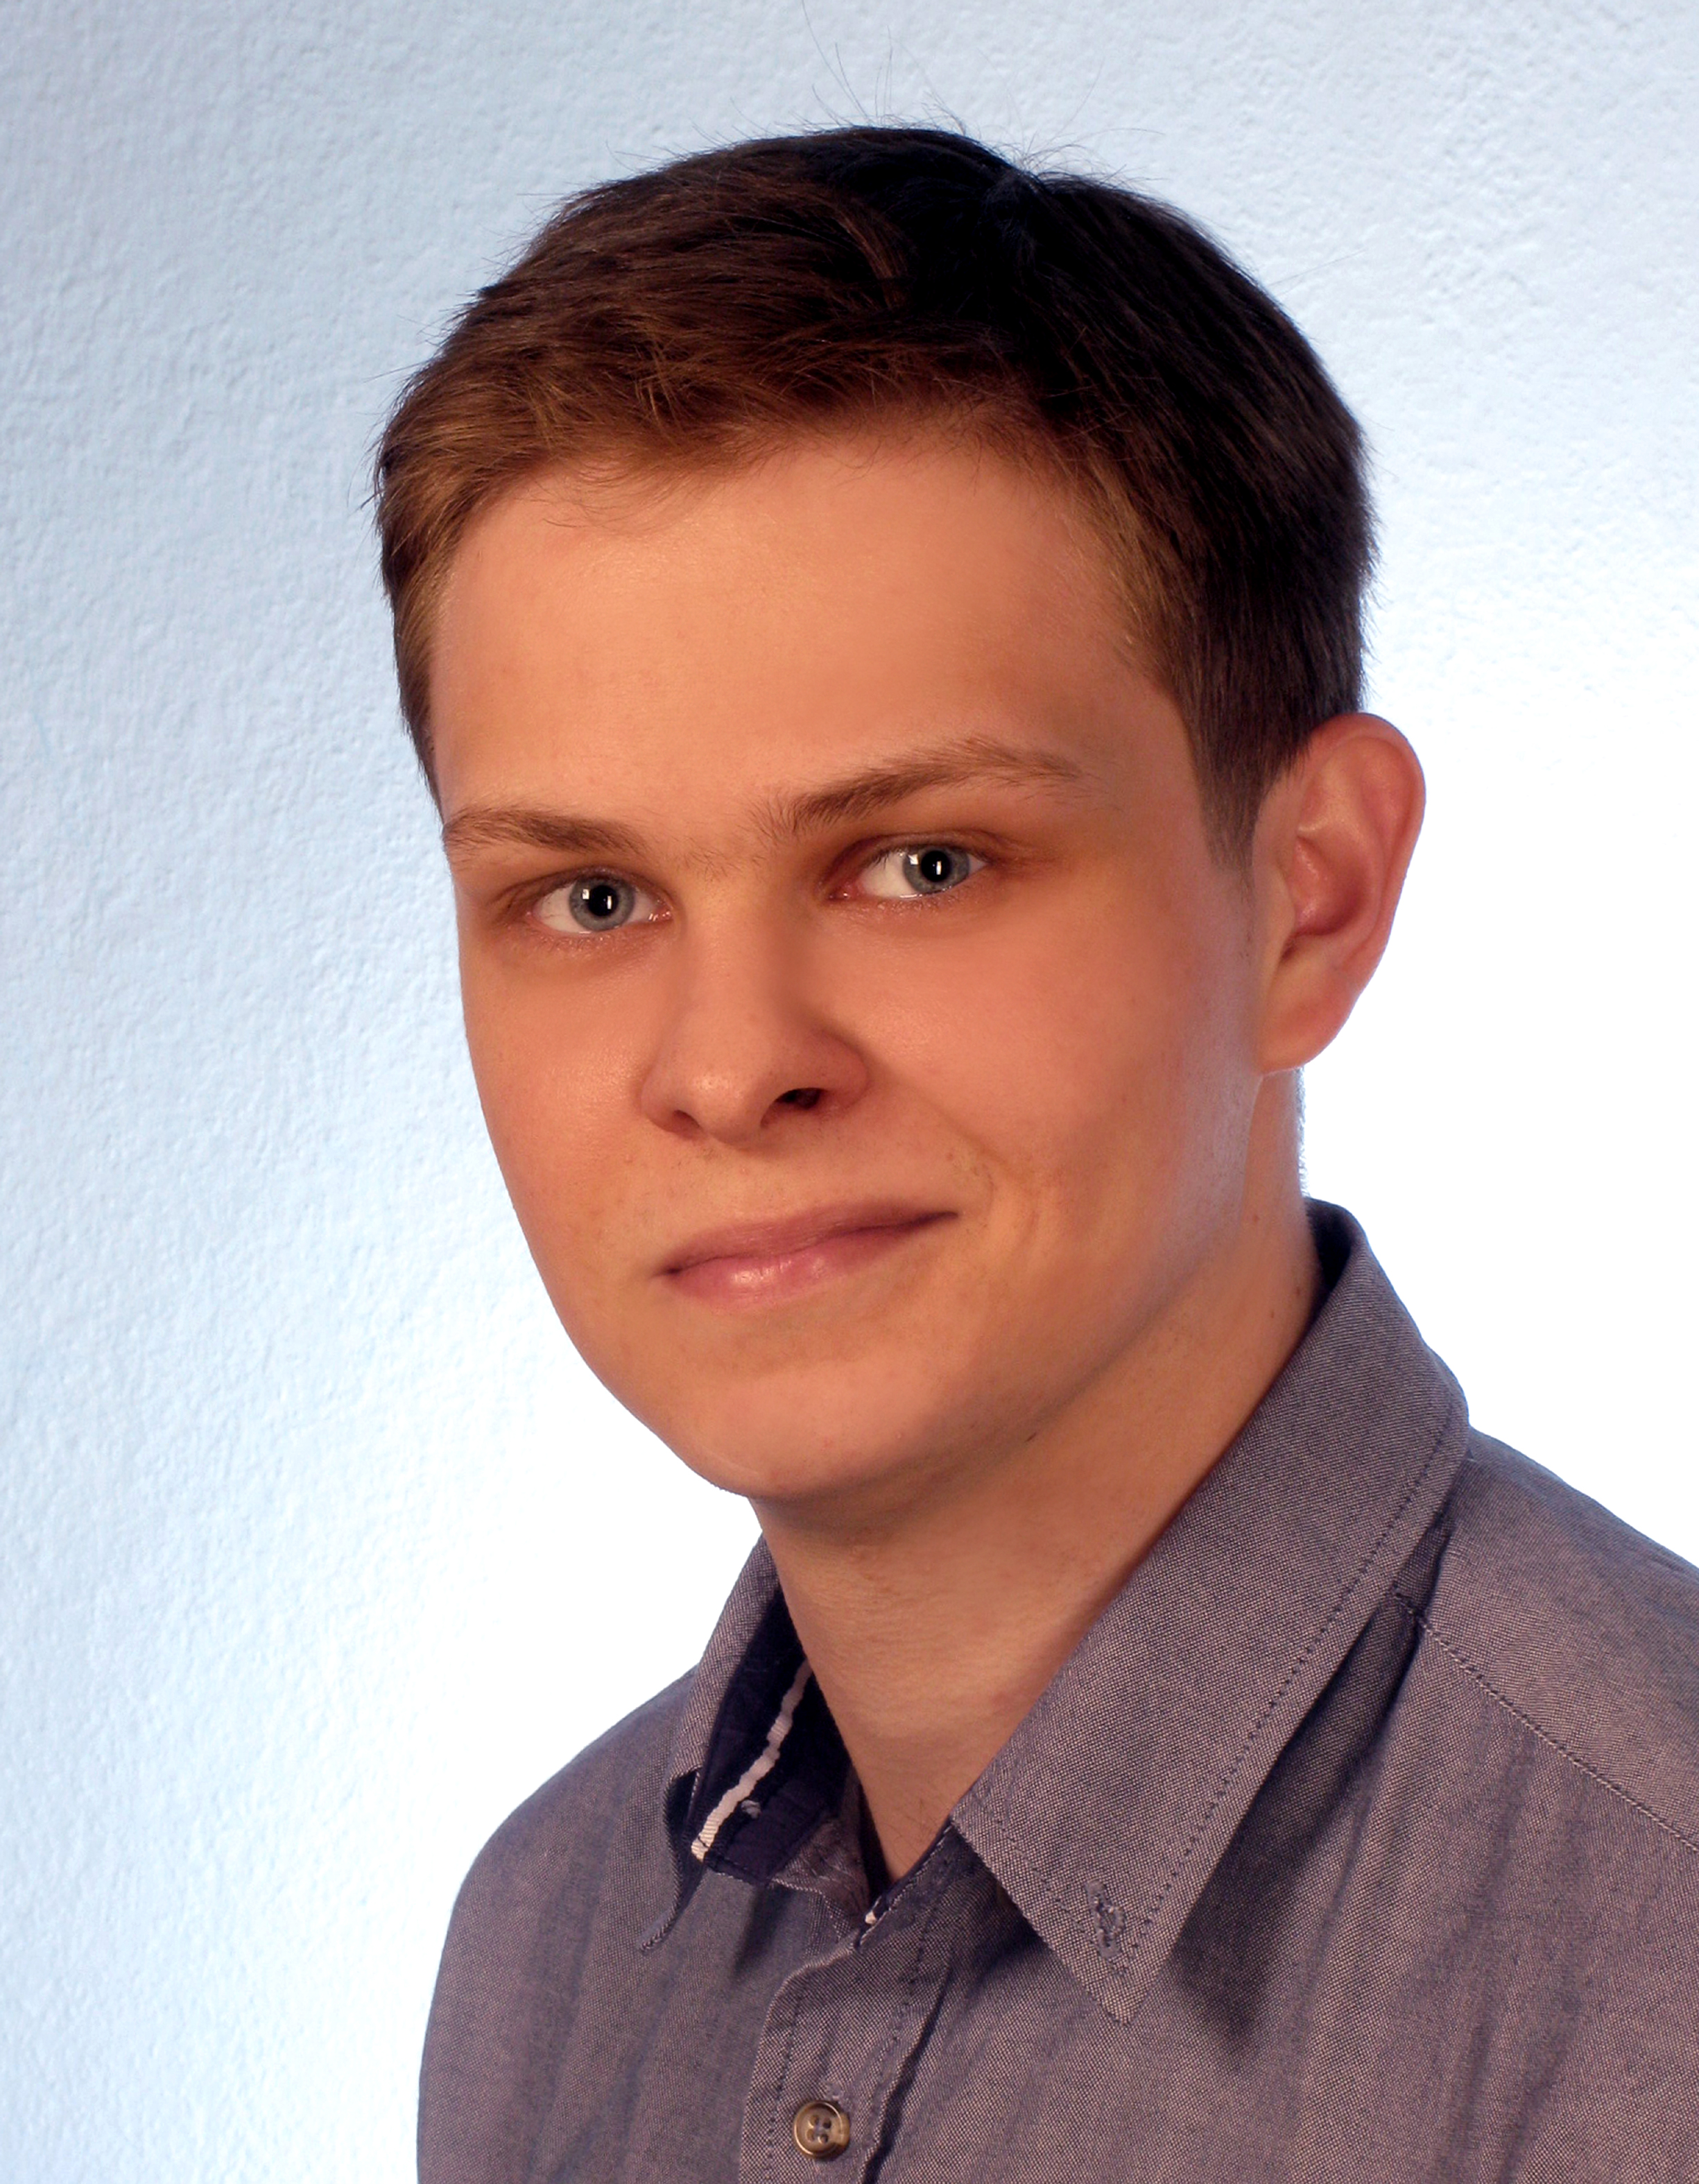
\includegraphics[height=5.0cm,width=4.0cm]{img/profile.jpg}
		\end{flushleft}
	\end{minipage}
	&
	\begin{minipage}{12cm}
		\begin{flushleft}
			\par\noindent\vspace{1\baselineskip}
			\begin{tabular}[h]{l r}
				{\normalsize\it Kierunek:} & \ \ \ \ \ \ \ \ \ \ \ \ \ \ \ \ \ \ \ \ \ \ \ \ \ \ \ \ \ \ \ \ \ \ \ \ \ \ \ \ \ \ \ Informatyka
			\end{tabular}
			\par\noindent\vspace{1\baselineskip}
			\begin{tabular}[h]{l r}
				{\normalsize\it Specjalność:} & Inżynieria Systemów Informatycznych
			\end{tabular}
			\par\noindent\vspace{1\baselineskip}
			\begin{tabular}[h]{l r}
				{\normalsize\it Data rozpoczęcia studiów:} & {\normalsize \ \ \ \ \ \ \ \ \ \ \ \ \ \ \ \ \ 24.02.2014 r.}
			\end{tabular}
			\par\noindent\vspace{1\baselineskip}
		\end{flushleft}
	\end{minipage}
\end{tabular}

\vspace*{1\baselineskip}
\begin{center}
{\large\bfseries Życiorys}\par\bigskip
\end{center}

\indent
Nazywam się Krzysztof Lis. Urodziłem się 19 czerwca 1991 roku w Nowym Jorku. W 2010 roku rozpocząłem studia na Wydziale Mechatroniki Politechniki Warszawskiej na kierunku Automatyka i Robotyka. I stopień studiów skończyłem na specjalności Automatyka z wyróżnieniem ``Summa Cum Laude'' przyznawanym przez Rektora Politechniki Warszawskiej. W ramach pracy inżynierskiej współpracowałem z firmą Siemens nad robotyzacją procesu paletyzacji. Podczas pracy nad projektem jako pierwszy w Polsce wykorzystałem środowisko Tecnomatix RobotExpert® wprowadzone przez firmę Siemens. Po uzyskaniu tytułu inżyniera rozpocząłem studia II stopnia na Wydziale Elektroniki i Technik Informacyjnych na kierunku Informatyka. W trakcie studiów pracowałem w warszawskim start-upie projektującym system dla centrum obrabiarkowego oraz rozpocząłem pracę jako programista w dziale technologii banku inwestycyjnego Goldman Sachs, gdzie miałem okazję brać udział w projektach prowadzonych w Polsce, Stanach Zjednoczonych oraz Wielkiej Brytanii.
\par
\vspace{2\baselineskip}
\hfill\parbox{15em}{{\small\dotfill}\\[-.3ex]
\centerline{\footnotesize podpis studenta}}\par
\vspace{3\baselineskip}
\begin{center}
	{\large\bfseries Egzamin dyplomowy} \par\bigskip\bigskip
\end{center}
\par\noindent\vspace{1.5\baselineskip}
Złożył egzamin dyplomowy w dniu \dotfill 20\_\_r.
\par\noindent\vspace{1.5\baselineskip}
z wynikiem \dotfill
\par\noindent\vspace{1.5\baselineskip}
Ogólny wynik studiów \dotfill
\par\noindent\vspace{1.5\baselineskip}
Dodatkowe wnioski i uwagi Komisji \dotfill
\par\noindent\vspace{1.5\baselineskip}
\dotfill



% Streszczenie
\newpage\thispagestyle{empty}
\vspace*{2\baselineskip} 
\begin{center}
	{\large\bfseries Streszczenie}\par\bigskip
\end{center}

{\itshape
Celem pracy magisterskiej jest omówienie teorii zagadnienia oceny ryzyka kredytowego w oparciu o dane historyczne. Przeprowadzono analizę danych pochodzących z platformy Lending Club®, na podstawie której dobrano model uczenia maszynowego obliczający prawdopodobieństwo niespłacenia pożyczki w oparciu o dane historyczne. Wybrany model został wykorzystany jako komponent przykładowej aplikacji web'owej umożliwiającej użytkownikowi przegląd statystyk pożyczek oraz ocenę ryzyka kredytowego dla danej pożyczki. W celu poprawy skalowalności aplikacji, uniezależnienia jej od środowiska w jakim jest uruchamiana oraz przystosowania do pracy w chmurze wykorzystano technologię kontenerów aplikacyjnych. 
}
\vspace*{1\baselineskip}

\noindent{\bf Słowa kluczowe}: {\itshape web, kontenery aplikacyjne, ryzyko kredytowe, systemy wspomagające podejmowanie decyzji, machine learning}
\par
\vspace{4\baselineskip}
\begin{center}
	{\large\bfseries The design of the web application supporting credit risk evaluation based on historic data.}\par\bigskip
\end{center}

{\itshape
This thesis picks up on the topic of the credit risk evaluation based on historic data. The author conducted a thorough analysis of data published by Lending Club in order to select an appropriate machine learning model, that would estimate the probability of default for a given loan. This component became the core of a sample web application, that allows users to view loan statistics and assess the credit risk of a particular loan. The scalability, environment isolation and cloud-compatibility issues were addressed by incorporating the application containers technology into the project.}
\vspace*{1\baselineskip}

\noindent{\bf Keywords}: {\itshape web, application containers, credit risk, decision support systems, machine learning}

\end{titlepage}


\end{document}
	
	\tableofcontents
	% \addcontentsline{toc}{chapter}{{Przedmowa1}{vii}}{vii}
	
	% \chapter*{Spis tablic, rysunków i~wydruków}
	% \listoftables
	% \listoffigures
	% \lstlistoflistings
	
	%\setlength{\baselineskip}{7mm}
	\newpage
	\pagenumbering{arabic}
	\setcounter{page}{1}
	
	\chapter{Wprowadzenie}

\section{Ocena ryzyka kredytowego}
Ocena ryzyka kredytowego jest kluczowym zagadnieniem z punktu widzenia współczesnych gospodarek rynkowych. Istnieje wiele różnych metod i narzędzi wykorzystywanych przez instytucje finansowe do oszacowania zdolności kredytowej partnera biznesowego – współcześnie tym zadaniem zajmują się wyspecjalizowane systemy informatyczne wykorzystujące osiągnięcia z dziedziny eksploracji danych. W ramach tej publikacji zostaną przedstawione podstawowe pojęcia związane z oceną ryzyka kredytowego, metody modelowania tego ryzyka wykorzystywane przez banki oraz zostanie zaprezentowana koncepcja platformy wspomagającej podejmowanie decyzji związanych z problemem oceny ryzyka kredytowego dla pożyczek typu P2P dostarczanych przez platformę Lending Club.

\section{Cel pracy}
Celem pracy jest przedstawienie roli oceny ryzyka kredytowego we współczesnych instytucjach finansowych, omówienie znaczenia tego zagadnienia na podstawie kryzysu na rynkach finansowych w latach 2007-2015 oraz zaproponowanie rozwiązań technologicznych wspomagających proces podejmowania decyzji w tym obszarze. W tym celu dokonano analizy danych pożyczkowych udostępnianych przez firmę Lending Club, na podstawie której dobrano model uczenia maszynowego służący jako model obliczeniowy w przykładowej implementacji systemu wspierającego ocenę ryzyka kredytowego.

\section{Struktura pracy}
Praca składa się z sześciu rozdziałów, z których pierwszy stanowi niniejszy wstęp.
\begin{description}
\item [Rozdział drugi] opisuje teorię zagadnienia oceny ryzyka kredytowego. Omówiona została rola działów zajmujących się tym problem w instytucjach finansowych, a także przeprowadzono analizę kryzysu na rynkach finansowych w latach 2007-2015, jako przykładu konsekwencji błędnego modelowania tego ryzyka. 
\item [Rozdział trzeci] został poświęcony analizie danych pożyczkowych udostępnianych przez platformę Lending Club oferującą pożyczki w systemie \textit{peer-to-peer}. Na podstawie przeprowadzonej analizy  wybrano statystyki prezentowane w ramach implementowanego systemu oraz dobrano model uczenia maszynowego, wyliczający prawdopodonieństwo niespłacenia pożyczki.
\item [W rozdziale czwartym] przedstawiono i porównano 3 rodzaje modeli służących do obliczania regresji logistycznej. W oparciu o analizę danych opisaną w poprzednim dziale dobrano parametry, na podstawie których przeprowadzono proces uczenia modeli, a następnie wybrano najlepszy z nich z uwzględniem środowiska aplikacji webowej, w jakiej będzie osadzony. 
\item [Rozdział piąty] omawia zagadnienie konteneryzacji aplikacji rozproszonych na przykładzie rozwiązania Docker, które  zostało wykorzystane przy implementacji systemu. Technologia ta zostałą wykorzystana ze względu na możliwość odizolowania aplikacji od środowiska serwera na jakim jest uruchamiania, co jest szczególnie istotne w przypadku aplikacji webowych uruchamianych w chmurze.
\item [W rozdziale szóstym] przedstawiono przykładową implementację systemu wspomagającego ocenę ryzyka kredytowego, opartego o przeprowadzoną wcześniej analizę. Omówione zostały nowoczesne technologie wykorzystane przy tworzeniu tej aplikacji.
\item [Rozdział siódmy] jest ostatnim rozdziałem pracy zawierającym jej podsumowanie oraz wnioski końcowe. 
\end{description}
 
	\chapter{Ryzyko kredytowe}

\section{Rola oceny ryzyka kredytowego we spółczesnych gospodarkach rynkowych}

\subsection{Wprowadzenie}

Wraz z postępem globalizacji, międzynarodowe rynki finansowe utworzyły strukturę przypominającą sieć naczyń połączonych. Zdarzenia występujące nawet w obrębie gospodarek pojedynczych państw mogą mieć znamienny wpływ na ogólnoświatową kondycję ekonomiczną. Biorąc pod uwagę, że stan współczesnych rynków ekonomicznych jest silnie skorelowany z kondycją instytucji finansowych takich jak banki, których główna działalność opiera się na kredytowaniu podmiotów zarówno prywatnych i instytucjonalnych, można jednoznacznie stwierdzić, że prawidłowa i precyzyjna ocena ryzyka kredytowego jest rzeczą absolutnie niezbędną z punktu widzenia zachowania równowagi na rynkach finansowych.

Przykładem katastrofalnych skutków, jakie niesie za sobą błąd w modelowaniu tego typu ryzyka jest wielki kryzys finansowy przypadający na lata 2007 – 2015, który zostanie dokładniej opisany w dalszej części artykułu. Ze względu na istotność i wagę tego problemu istnieje szereg dyrektyw międzynarodowych nakładających stosowne regulacje na instytucje finansowe, aby stosowane przez nie praktyki w sferze kredytowania nie mogły doprowadzić do poważnych zachwiań w gospodarkach światowych na miarę wspomnianego kryzysu.

Najbardziej istotnymi dokumentami tego typu są normy Basel II i Basel III wprowadzone przez Basel Comittee on Banking Supervision (BCBS) – organ powołany przez banki centralne sprawujący szeroko pojęty nadzór nad praktykami całego sektora bankowego.

\subsection{Definicja ryzyka kredytowego}

Ryzykiem kredytowym nazywamy ryzyko zaistnienia takich okoliczności, z powodu których wartość portfela kredytów i papierów wartościowych instytucji ulegnie wahaniom (spadkowi) z powodu nagłych i nieprzewidzianych zmian zdolności kredytowej kredytobiorców lub partnerów inwestycyjnych.

Podstawowym podziałem ryzyka kredytowego jest:
\begin{itemize}
\item Ryzyko niewypłacalności, czyli wystąpienia opóźneń bądź całkowitego zaprzestania spłaty kredytu
\item Ryzyko spadku zdolności kredytowej (Credit Ratings)
\end{itemize}

Z punktu widzenia projektowania platformy wspomagającej ocenę ryzyka kredytowego istotna jest ta druga podgrupa.

\subsection{Metody oceny ryzyka kredytowego}

Kluczową miarą z punktu widzenia zarządzania ryzykiemr kredytowym jest RWA - Risk-weighted Assets. RWA składa się z:

\begin{itemize}
\item Sumy wag ryzyka pomnożonych przez kapitał pozycji uwzględnainej w bilansie
\item Sumy wag ryzyka pomnożonych przez
ekwiwalent kredytu dla pozycji nie uwzględnianej w bilansie (np. instrumenty pochodne)
\end{itemize}

\begin{equation} \label{eq:RWA}
RWA = \sum_{i=1}^{N}\alpha_{i}E_{i} + \sum_{j=1}^{M}w_{j}C_{j}
\end{equation}
Gdzie:
\begin{itemize}
	\item $\alpha_{i}$ - waga ryzyka dla i-tej pozycji uwzględnianej w bilansie
	\item $E_{i}$ - kapitał i-tej pozycji uwzględnianej w bilansie
	\item $w_{j}$ - waga ryzyka dla j-tej pozycji nie uwzględnianej w bilansie
	\item $C_{j}$ - ekwiwalent kredytu dla j-tej pozycji nie uwzględnianej w bilansie
\end{itemize}

Formuła (\ref{eq:RWA}) jest najbardziej ogólną formą modelu służącego bankom do wyznaczenia wartości RWA. Następnie w oparciu o tę wartość wyznaczany jest wymagany kapitał zabezpieczający udzielone kredyty – stanowi on 8\% RWA. Istnieją dwa podstawowe podejścia do zagadnienia modelowania ryzyka:

\begin{itemize}
\item Podejście standaryzowane (ang. \textit{Standardized Approach})
\item Podejście oparte na wewnętrznym ratingu (ang. \textit{Internal-Rating Based Approach})
	\begin{itemize}
	\item Foundation IRB
	\item Advanced IRB
	\end{itemize}
\end{itemize}

\subsubsection{Standardized approach}

Wartości wag do wzoru (\ref{eq:RWA}) dostarcza krajowy regulator. Są one zdefiniowane dla poszczególnych klas kredytobiorców, np. korporacja, bank, instytucja rządowa. Jest to najprostsza forma wyznaczania wartości RWA stosowana jedynie przez mniejsze instytucje, które nie mogą sobie pozwolić na stosowanie bardziej zaawansowanych metod modelowania ryzyka.

\subsubsection{Internal-RatingBasedApproach}
W przypadku wariantu “Foundation” bank musi wyznaczyć jedynie prawdopodobieństwo niewypłacalności (ang. \textit{Probability of Default}), natomiast w przypadku metody zaawansowanej (Advanced IRB) oprócz PD bank musi wyznaczyć stratę przy (całkowitej) niewypłacalności (ang. \textit{Exposure at Default}) oraz faktyczną stratę (ang. Loss Given Default), która określa procentowy stosunek poniesionych strat do straty przy niewypłacalności (EAD). Otrzymane wartości pozwalają na wyznaczenie wartości RWA w oparciu wewnętrzy model banku, pod warunkiem, że jego specyfikacja została dostarczona krajowemu regulatorowi oraz pomyślnie przeszła weryfikację poprawności i zgodności z obowiązującymi normami.

\section{Kryzys na światowych rynkach finansowych po roku 2007}

\subsection{Geneza}

Genezy gólnoświatowego kryzysu gospodarczego rynków finansowych należy szukać na rynku pożyczek wysokiego ryzyka udzielanych w USA osobom o niewystarczających możliwościach finansowych (ang. subprime mortgage). Pożyczki te były wykorzystywane jako zabezpieczenie obligacji strukturyzowanych emitowanych przez instytucje finansowe – w szczególności duże banki. Z powodu hossy na rynku nieruchomości i wprowadzenia mniej restrykcyjnych przepisów prawnych, instytucje ratingowe wystawiały rzeczonym obligacjom zawyżone oceny. Ponadto na rynku amerykańskim występowały silne naciski polityczne – ze strony administracji Billa Clintona, a następnie George’a W. Busha – mające na celu rozszerzenie grona potencjalnych kredytobiorców o osoby znajdujące się w gorszej sytuacji ekonomicznej.

\subsection{Przebieg}

Skutkiem nadmiernego rozluźniania polityki pieniężnej było wystąpienie symptomów przegrzania amerykańskiej gospodarki. W obawie przed gwałtownym wzrostem inflacji FED zdecydował się na podniesienie stóp procentowych – z poziomu 1\% w 2004 roku do 5,25\% w 2006 roku. Przełożyło się to bezpośrednio na zwiększenie odsetek, jakimi byli obciążeni kredytobiorcy. Doprowadziło to do zachwiania na rynku nieruchomości – wiele osób traktowało taki zakup jako inwestycję finansowaną za pomocą kredytu. W momencie kiedy spadł popyt zaczęły spadać ceny nieruchomości, co stało się przyczynkiem problemów kredytobiorców. Banki, w obliczu zaprzestania spłat kredytów, zaczęły zajmować hipoteki i masowo sprzedawać przejęte nieruchomości. Poskutkowało to gwałtowną akceleracją spadku cen i spiralnym nawarstwianiem się problemów gospodarki amerykańskiej.

Instytucje finansowe poniosły gigantyczne straty, a wiele z nich stanęło na skraju bankructwa. Rząd amerykański zdecydował się dokapitalizować największe banki w obawie przed kryzysem porównywalnym do kryzysu stulecia z lat 30. Jeden z największych banków inwestycyjnych na świecie, Lehman Brothers, otrzymał odmowę przyznania pomocy od banku centralnego USA i ogłosił upadłość. Zasiało to panikę na rynku finansowym i zapoczątkowało serię nerwowych i pochopnych decyzji, które doprowadziły między innymi to dodruku taniego pieniądza, wzrostu inflacji i deregulacji rynku finansowego.

\subsection{Skutki kryzysu}

Oprócz gwałtownego spadku cen (20 – 30\%) na rynku nieruchomości w Stanach Zjednoczonych, spowolnienie gospodarcze dotknęło wielu krajów na świecie. Brak zaufania wobec instytucji finansowych spowodował ucieczkę inwestorów w kierunku innych branż oraz falę spekulacji.

\begin{figure}[h] \centering %H if want to get it exaclty here
	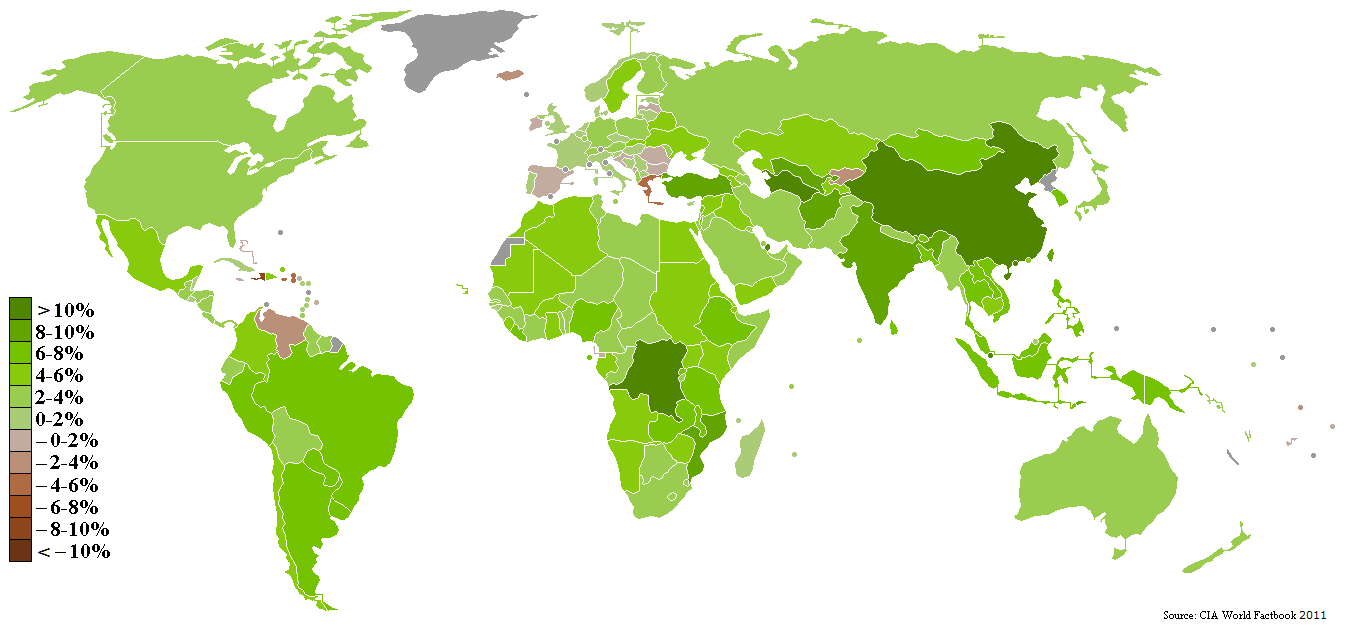
\includegraphics{img/gdp_rate_2007.png}
	\caption{Wzrost PKB w poszczególnych państwach w 2007 roku.\cite{CIA}}
	\label{abcCode}
\end{figure}

Wzajemna nieufność instytucji finansowych poskutkował wstrzymaniem akcji kredytowej i zamrożeniem inwestycji. Światowe gospodarki pogrążyły się w recesji, czyli charakteryzował je ujemny przyrost PKB (kurczenie się gospodarki). Najmniej zostały dotknięte kraje arabskie, które w dużej mierze bazują na eksporcie surowców.

\subsubsection{Wpływ na rynek surowców naturalnych}

\begin{figure}[h] \centering %H if want to get it exaclty here
	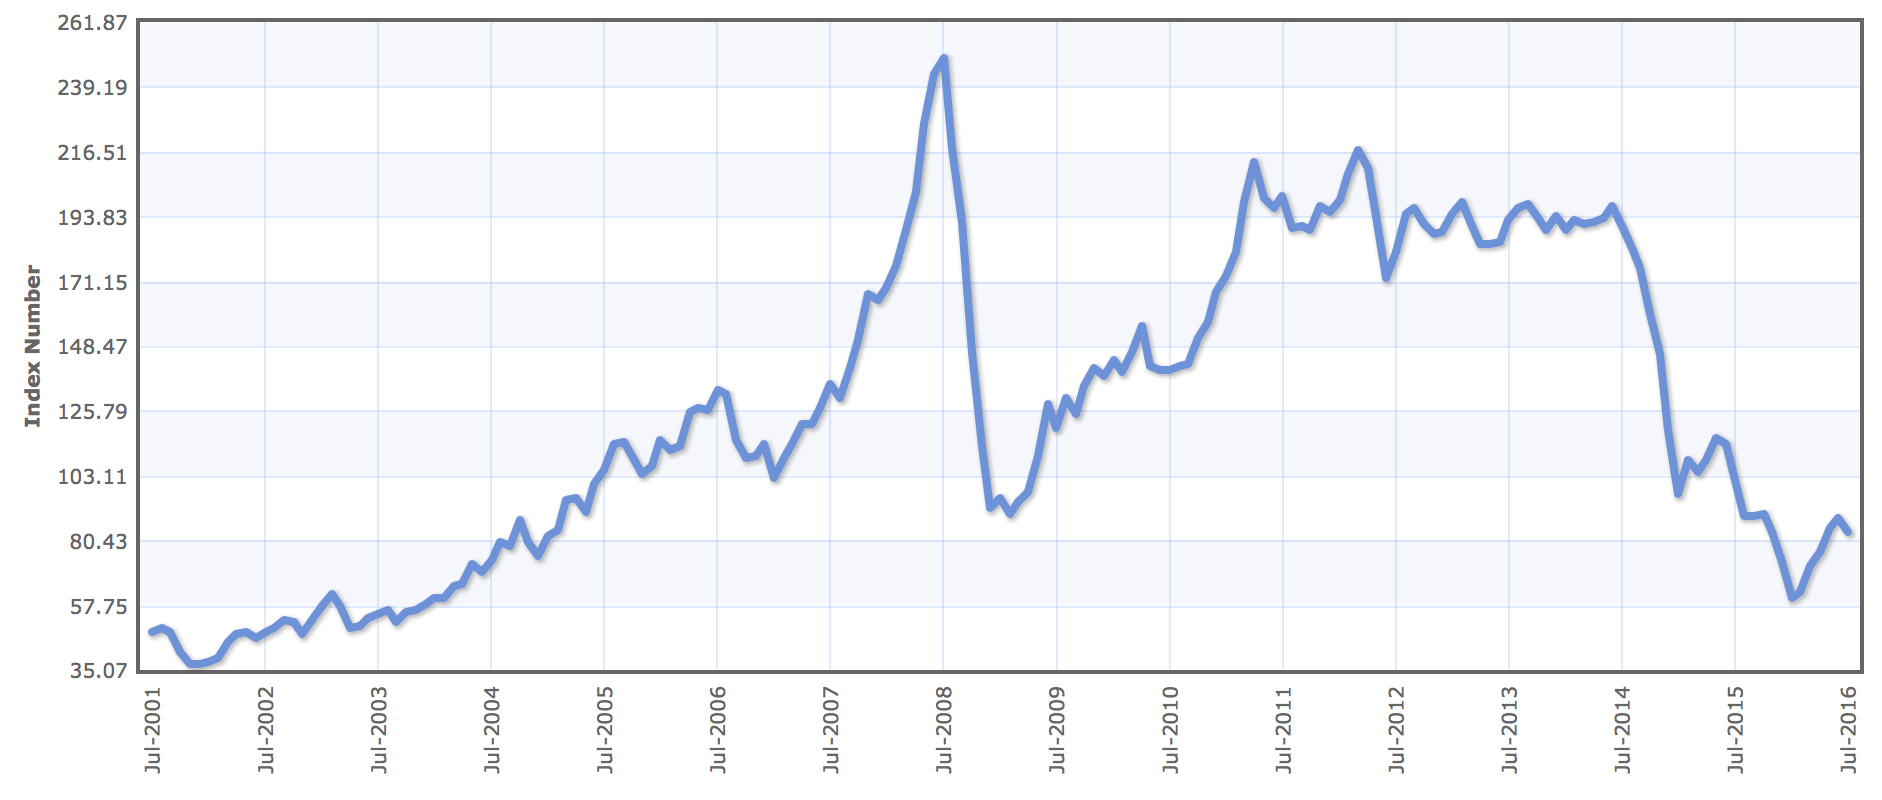
\includegraphics[scale=0.4]{img/fuel_index.png}
	\caption{Indeks cen paliw kopalnych latach 2001 - 2016.\cite{indexmundi}} %indexmundi.com
	\label{fuelPriceIndex}
\end{figure}

\begin{figure}[h] \centering %H if want to get it exaclty here
	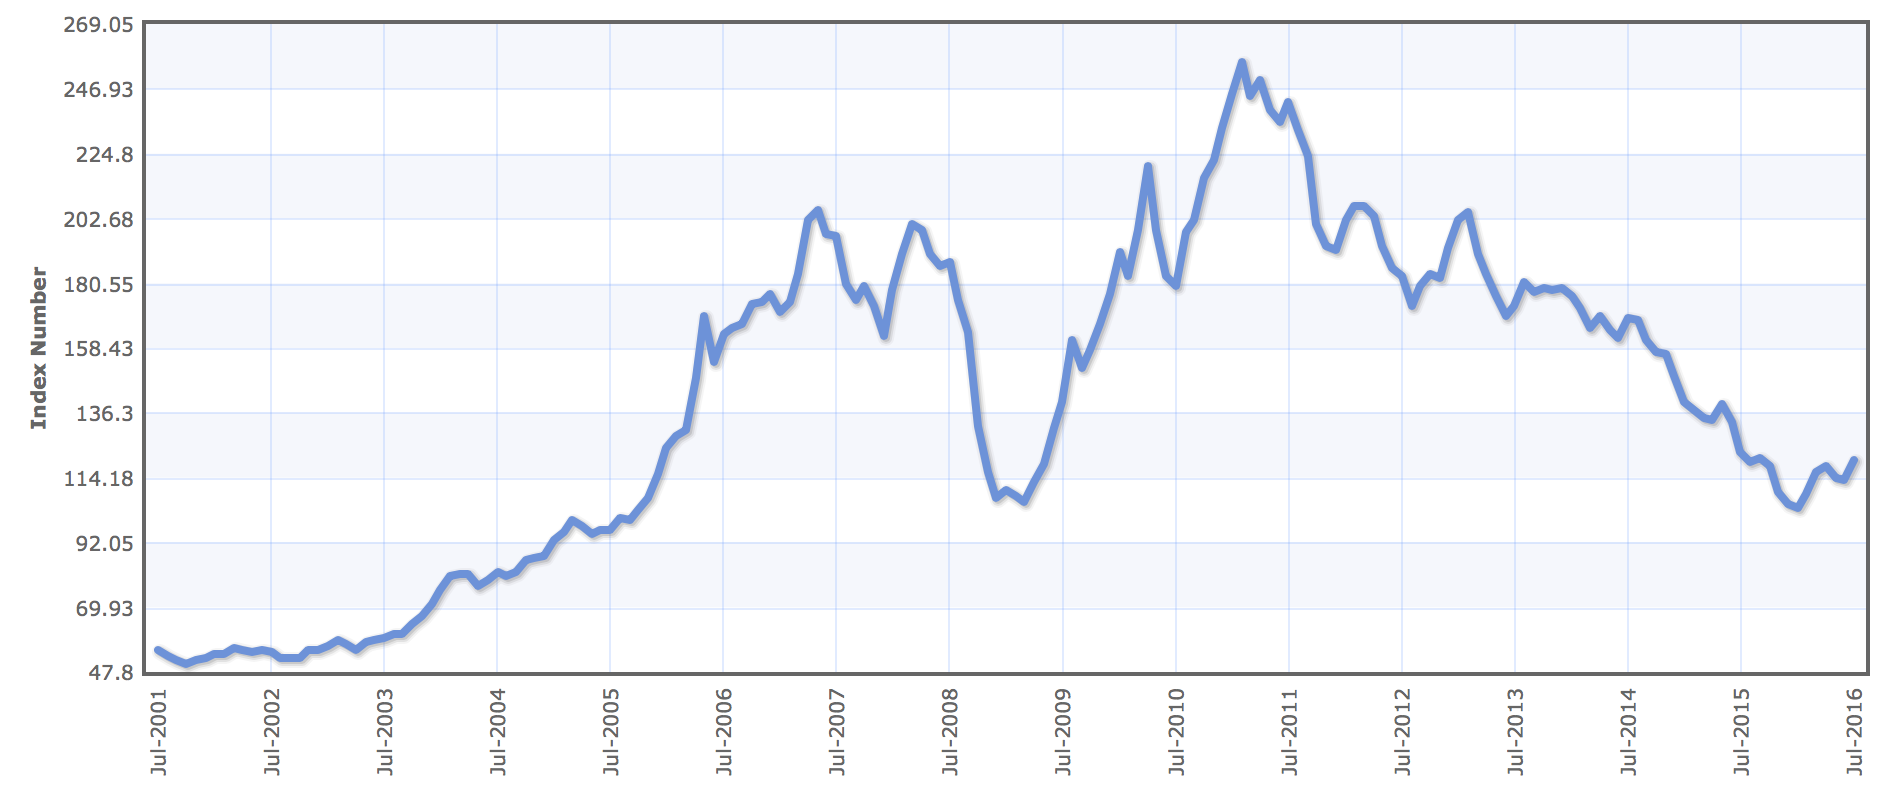
\includegraphics[scale=0.4]{img/metal_index.png}
	\caption{Indeks cen metali latach 2001 - 2016.\cite{indexmundi}} %indexmundi.com
	\label{metalPriceIndex}
\end{figure}

Wykresy przedstawione na rysunkachh 2.2 i 2.3 ukazują gwałtowny wzrost zainteresowania inwestycjami opartymi na surowcach naturalnych. Doprowadziło to do nienaturalnego, lecz chwilowego wzrostu cen - cena baryłki ropy wzrosła niemalże trzykrotnie na przestrzeni 18 miesięcy. Niestety ze względu na zamrożenie wielu inwestycji spowodowane brakiem kredytów po skoku cen nastąpił równie raptowny ich spadek. Przysporzyło to wielu problemów przedsiębiorstwom wydobywczym, m.in. doprowadziło do bankructwa wiele australijskich kopalni niklu.

\subsubsection{Wpływ na ceny żywności}

\begin{figure}[h] \centering %H if want to get it exaclty here
	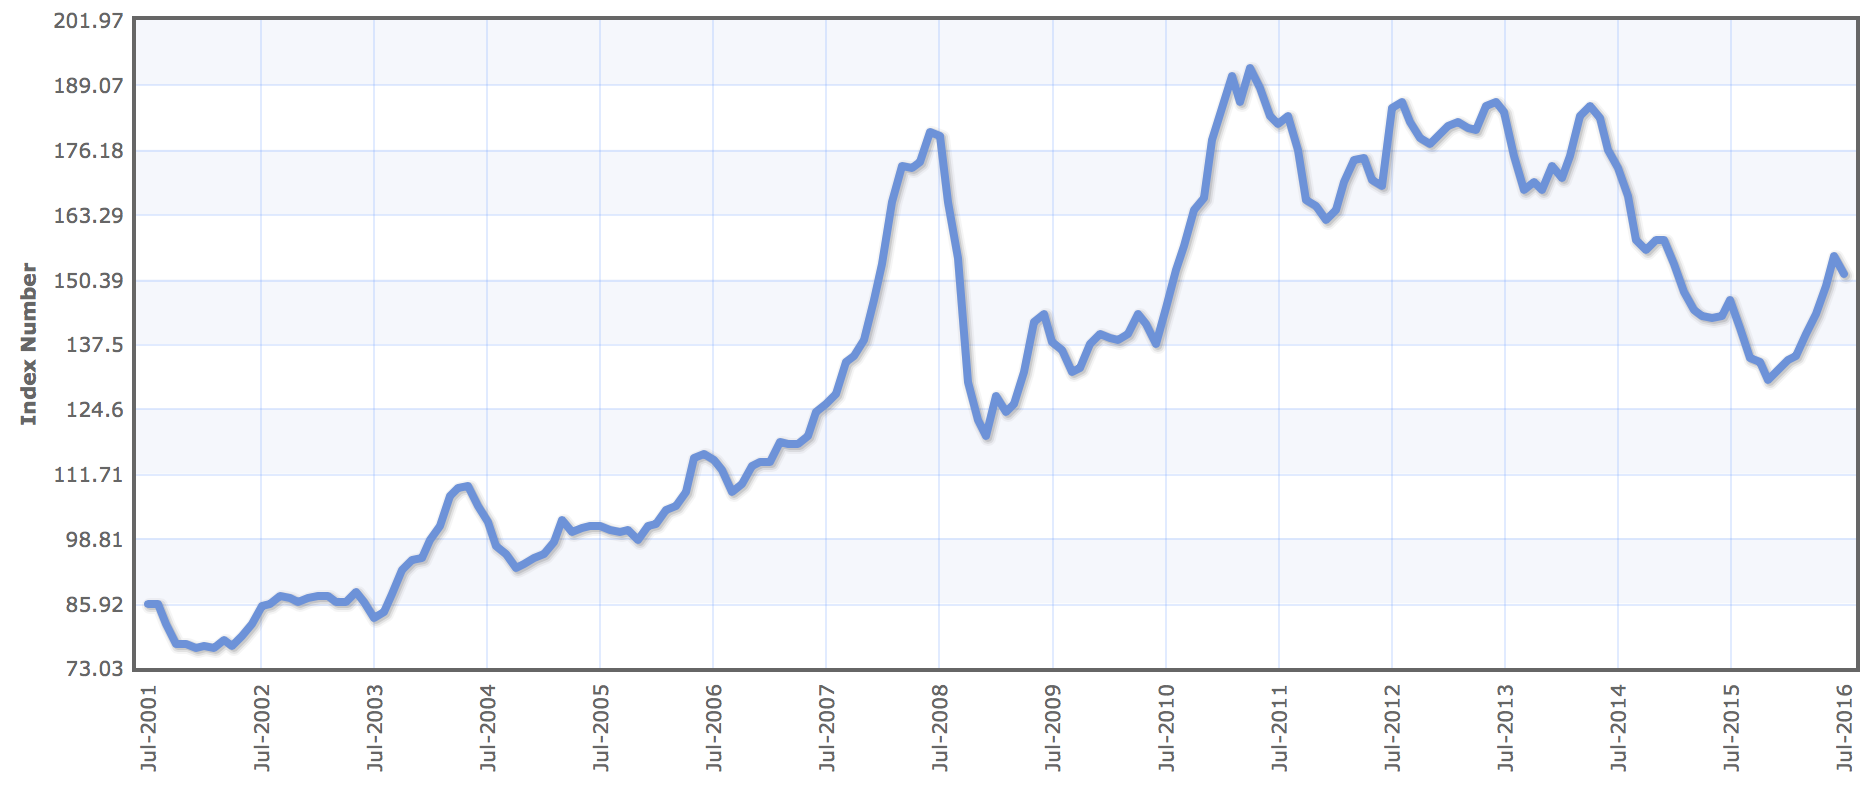
\includegraphics[scale=0.4]{img/food_index.png}
	\caption{Indeks cen żywności latach 2001 - 2016.\cite{indexmundi}} %indexmundi.com
	\label{foodPriceIndex}
\end{figure}

Jednym z tragicznych następstw kryzysu na rynkach finansowych był radykalny wzrost cen żywności. Najbardziej odczuły to kraje rozwijające się i tzw. Kraje Trzeciego Świata. Doprowadziło to do politycznej i ekonomicznej niestabilności w tych regionach.

\subsubsection{Bezrobocie}

Wzajemna nieufność instytucji finansowych poskutkował wstrzymaniem akcji kredytowej i zamrożenia inwestycji. Światowe gospodarki pogrążyły się w recesji, czyli charakteryzował je ujemny przyrost PKB (kurczenie się gospodarki). Najmniej zostały dotknięte kraje arabskie, które w dużej mierze bazują na eksporcie surowców.
za masowymi zwolnieniami w sektorze finansowym (w samej Wielkiej Brytanii pracę w tym sektorze straciło kilkadziesiąt tysięcy osób) ucierpiały również inne branże – przede wszystkim branża motoryzacyjna. Było to spowodowane załamaniem sprzedaży nowych samochodów finansowanej głównie za pomocą kredytów – a banki przestały ich udzielać.
Zadłużenie społeczeństwa i rosnące bezrobocie spowodowały spadek konsumpcji, co w sposób spiralny prowadziło do dalszego spadku produkcji i redukcji zatrudnienia.

\subsection{Walka z kryzysem}

Walka z kryzysem w dużej mierze sprowadzała się do dotowania instytucji sektora finansowego z pieniędzy podatników oraz stosowania praktyk protekcjonistycznych w stosunku do rodzimych firm – szczególnie dotyczyło to USA i Francji. W celu pobudzenia akcji kredytowej wprowadzono rekordowe obniżki stóp procentowych, co miało skłonić inwestorów do bardziej śmiałych i zdecydowanych działań.
Postanowiono wprowadzić nową normę: Basel III, która miała uchronić sektor finansowy przed popełnieniem tych samych błędów. Należy jednak pamiętać, że poprzednia odsłona tych regulacji – mylnie obwiniana za zaistniały kryzys – została ogłoszona w roku 2004, a w roku 2008 dopiero była wdrażana, czyli nie miała szansy realnie wpłynąć na kondycję ekonomiczną sektora bankowego i uchronić świata przed nadchodzącym gospodarczym tąpnięciem.
Rządy państw grupy G8 przekazały w sumie ponad 3 bln. \$ na cel ratowania własnych gospodarek. Postanowiono również zwiększyć rezerwy Międzynarodowego Funduszu Walutowego, a także planowano likwidację rajów podatkowych – pomysł ten nie doczekał się jednak realizacji.
	\chapter{Analiza danych pochodzących z serwisu Lending Club}

\section{Opis platformy Lending Club}

Lending Club to amerykański startup finansowy utworzony w 2006 z główną siedzibą znajdującą się w San Francisco, w stanie Kalifornia. Firma jest dostawcą platformy oferującej pożyczki w formacie \textit{peer-to-peer} - pożyczkobiorcy mogą pozyskiwać finansowanie bezpośrednio u potencjalnych pożyczkodawców, bez udziału instytucji postronnych \cite{LendingClub}. Jest to pierwsza spółka tego sektora, która zarejstrowała swoje produkty w amerykańskiej komisji papierów wartościowych (ang. \textit{US Securities and Exchange Comission}). Wszystkie operacje prowadzone są w ramach platformy internetowej, co pozwoliło na znaczną redukcję kosztów z jakimi muszą mierzyć się tradycyjne instytucje finansowe (np. koszty związane z utrzymywaniem placówek). Dzięki temu stopy procentowe przypisane do pożyczek są atrakcyjne zarówno dla kredytobiorców, jak i potencjalnych inwestorów. 

\subsection{Model biznesowy}

Założeniem Lending Club jest dostarczenie użytkownikom platformy, która umożliwi interakcję dwóm komplementarnym grupom - pożyczkobiorcom i inwestorom. Pożyczkobiorcy zgłaszają zapotrzebowanie na kredyt za pośrednictwem publicznie dostępnej listy pożyczek, przy czym kwota kredytu musi mieścić się w zakresie \$1000 - \$40000 a termin spłaty pożyczki musi wynosić 36 lub 60 miesięcy. Na podstawie danych użytkownia, zawierających informacje na temat jego historii kredytowej, bieżącej zdolności kredytowej, kwoty pożyczki o jaką się ubiega oraz jego stosunku zadłużenia do dochodu, pożyczce nadawany jest stopień z zakresu A-G (przy czym pożyczki oznaczone symbolem ``A'' oznaczają najniższy stopień ryzyka, a ``G'' najwyższy) oraz wyznaczana jest wysokość opłat i stopa zwrotu przypisana pożyczce \cite{LendingClub}. 

Inwestorzy mogą budować swoje portfolio ręcznie, wybierając pożyczki z dostępnej listy i określając kwotę inwestycj, lub korzystając z algorytmu automatycznie dobierającego zrównoważony portfel pożyczek. W przypadku podejmowania decyzji inwestycyjnych bezpośrednio przez inwestorów wzrasta znaczenie zewnętrznych systemów wspomagających podejmowanie decyzji. Taką rolę będzie pełnił system opracowany w ramach tej pracy magisterskiej - aplikacja będzie udostępniała użytkownikom statystyki wygenerowane na podstawie danych historycznych oraz moduł wyliczający prawdopodobieństwo niespłącenia pożyczki przez pożyczkobiorcę. W oparciu o te informacje dużo łatwiej jest zarządzać strategią inwestycyjną, polegającą na wczesnej sprzedaży pożyczek o zbyt wysokim ryzyku oraz skupowaniu pożyczek (dzięki predykcji z zastosowaniem algorytmów uczenia maszynowego, można określić to prawdopodobieństwo przed spadkiem wartości długu), które prawdopodobnie zostaną spłacone w terminie.

\section{Analiza udostępnionych danych}

Lending Club co kwartał publikuje dane opisujące pożyczki zawarte w poprzednim okresie rozliczeniowym wraz ze słownikiem opisującym te dane, który został załączony do tej pracy. Najpierw dokonano wstępnego przetworzenia danych, polegającego na:

\begin{itemize}
\item scaleniu danych z poszczególnych okresów w jeden plik
\item konwersji danych zawartych w następujących kolumnach do wartości numerycznych:
	\begin{itemize}
		\item int\_rate - stopa procentowa,
		\item revol\_util - procentowy skaźnik zużycia lini kredytowej,
		\item emp\_legth - długość zatrudnienia,
		\item term - okres spłaty pożyczki,
		\item pymnt\_plan - pożyczki, które mają rozpisany plan płatności zostały oznaczone wartością ``1'', w przeciwnym wypadku ``0''.
	\end{itemize}
\end{itemize}

Ponadto utworzono dodatkową kolumnę \textit{``defaulted''}, w której pożyczki uznane za niespłacone, tj. o statusie należącym do grupy: \textit{Charged Off, Default, Late (16-30 days), Late (31-120 days)}, zostały oznaczone wartością ``1'', a pozostałe wartością ``0''.

\subsection{Statystyki według stanu}

Bardzo istotną informacją z punktu widzenia inwestora jest popularność platformy w poszczególnych stanach. Na podstawie informacji na temat liczby pożyczek i łącznej kwoty, na którą zostały udzielone w poszczególnych stanach możliwe jest określenie potencjalnej liczby inwestorów i dynamikę rynku kredytowego w danym regionie. Dzięki tym danym inwestor jest świadomy, w jakim stopniu będzie mógł zarządzać długiem w przyszłości, np. czy łatwo będzie mu odsprzedać zadłużenie innemu inwestorowi. Kod generujący te statystyki został przedstawiony na Wydruku \ref{r:valueState} i \ref{r:volumeState}.

\begin{lstlisting}[language=R, caption={Skrypt wyliczający łączną kwotę udzielonych kredytów dla każdego stanu}, label={r:valueState}]
state_by_value <- loanbook %>% group_by(region) %>% 
	summarise(value = sum(loan_amnt, na.rm=TRUE))

state_choropleth(state_by_value, title = "Value by State")
\end{lstlisting}

\begin{figure}[h] \centering %H if want to get it exaclty here
	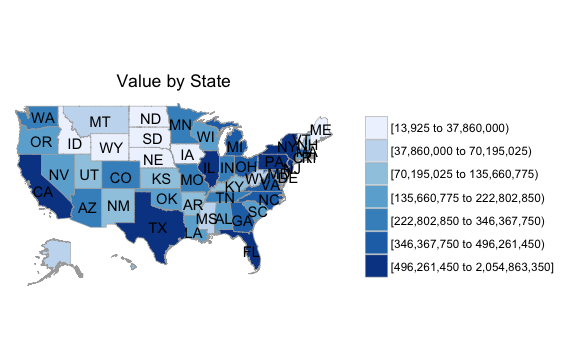
\includegraphics[scale=0.7]{img/value_state.png}
	\caption{Łączna kwota udzielonych kredytów wg. stanu.}
	\label{lc:value_state}
\end{figure}

Zarówno w przypadku liczby jak i łącznej kwoty udzielonych kredytów stanem o najwyższych statystykach jest Kalifornia. Wynika to przede wszystkim z zamożności społeczeństwa, ale również z faktu, że wiele firm technologicznych, w tym Lending Club, pochodzi właśnie z tego stanu i jest to rynek, na którym operują najdłużej i któremy poświęciły bardzo dużo uwagi. Usługi oferowane przez Lending Club cieszą się dużą popularnością w bogatych stanach, takich jak wspomniana Kalifornia, Teksas oraz stany wschodniego wybrzeża USA. Zdecydowanie mniej popularne są w uboższym rejonie północnych stanów USA. 

\begin{lstlisting}[language=R, caption={Skrypt wyliczający liczbę udzielonych kredytów dla każdego stanu}, label={r:volumeState}]
state_by_volume <- loanbook %>% group_by(region) %>%
  summarise(value = n())

state_choropleth(state_by_volume, title = "Volume by State")
\end{lstlisting}

\begin{figure}[h] \centering %H if want to get it exaclty here
	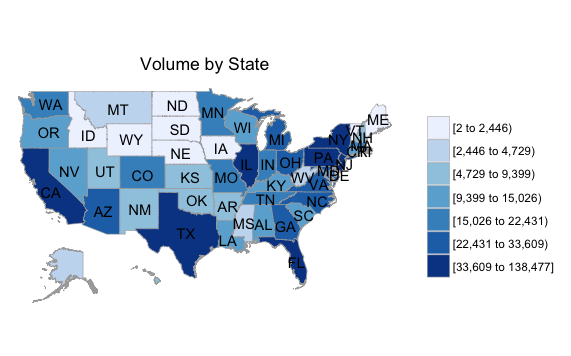
\includegraphics[scale=0.7]{img/volume_state.png}
	\caption{Liczba udzielonych kredytów wg. stanu.}
	\label{lc:volume_state}
\end{figure}

\subsection{Wysokość pożyczek}

Po zbadaniu rozkładu danych względem wysokości pożyczki (Rysunek \ref{lc:amnt_distrib}) okazało się, że mediana dla tych danych wynosi \$13225,00 a średnia wysokość \$14900,25. Obie te wartości są znacznie poniżej maksymalnego limitu wynoszącego \$40000 - ponadto 70\% wszystkich kredytów zostało udzielonych na kwotę nie większą niż \$20000, co stanowi połowę dopuszczalnego limitu.

\begin{figure}[h] \centering %H if want to get it exaclty here
	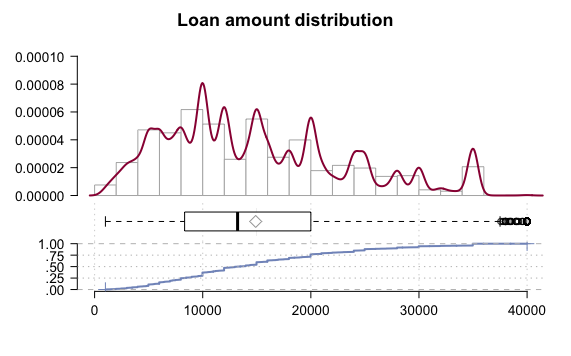
\includegraphics[scale=0.5]{img/loan_amt_distrib.png}
	\caption{Rozkład pożyczek względem ich wysokości.}
	\label{lc:amnt_distrib}
\end{figure}

Rysunek \ref{lc:amnt_growth} przedstawia wzrost ruchu na platformie na przestrzeni lat. Punktem przełomowym jest marzec 2014, kiedy firma weszła na giełdę - od tego czasu suma pożyczek zawartych na platformie uległa potrojeniu.

\begin{figure}[h] \centering %H if want to get it exaclty here
	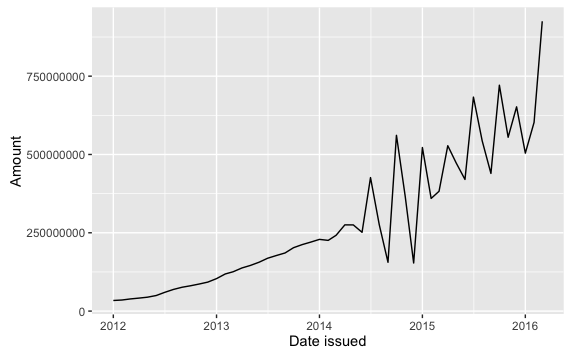
\includegraphics[scale=0.5]{img/loanbook_growth.png}
	\caption{Całkowita kwota pożyczek udzielonych w ramach Lending Club.}
	\label{lc:amnt_growth}
\end{figure}

\subsection{Powody zaciągania kredytów konsumenckich}

Wedlug serwisu Bankrate.com \cite{bankrate} najpopularniejsze powody zaciągania pożyczek konsumenckich w Stanach Zjednoczonych to:

\begin{itemize}
	\item konsolidacja długów,
	\item spłata kart kredytowych,
	\item remont domu,
	\item ślub,
	\item przeprowadzka,
	\item opłaty związane z pogrzebem bliskiej osoby,
	\item opłaty związane z leczeniem (w USA służba zdrowia nie ma charakteru publicznego),
	\item zakup samochodu,
	\item wakacje.
\end{itemize}

Znajduje to odzwieciedlenie w danych serwisu Lending Club (Rysunek \ref{lc:purposes}). Konsolidacja długów stanowi 59,5\% wszystkich zaciągniętych pożyczek, a druga pozycja w zestawieniu - spłata karty kredytowej - 23,8\%. Łącznie te dwie grupy stanowią ponad 80\% wszystkich kredytów. Jest to spowodowane nieustannym wzrostem zadłużenia społeczeństwa amerykańskiego - w 2015 roku całkowita kwota udzielonych kredytów konsumenckich wzrosła o 7\%, a w pierwszym kwartale 2016 o 5,8\% w stosunku do anologicznego okresu w ubiegłym roku \cite{federalreserve}.

\begin{figure}[h] \centering %H if want to get it exaclty here
	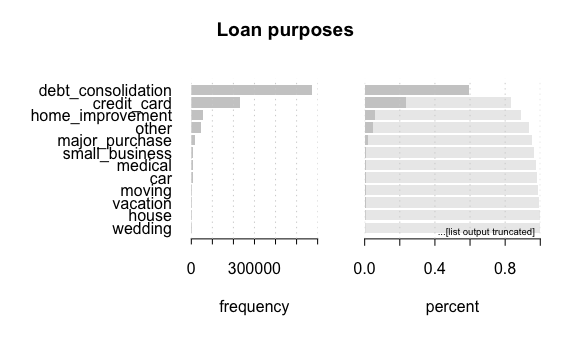
\includegraphics[scale=0.7]{img/purposes.png}
	\caption{Powody zaciągania pożyczek konsumenckich w Lending Club.}
	\label{lc:purposes}
\end{figure}

\subsection{Zdolność kredytowa użytkowników Lending Club}

Zdolność kredytowa użytkowników jest oceniana w siedmiostopniowej (Rysunek \ref{lc:grades}) skali na podstawie ich historii kredytowej oraz informacji o stanie zatrudnienia i posiadanych nieruchomościach. Najbezpieczniejsze pożyczki otrzymują kategorię A, natomiast te o największym stopniu ryzyka - G \cite{LendingClub}. Najliczniejszą grupę kredytów stanowią pożyczki o kategoriach B i C - w sumie stanowią prawie 60\% wszystkich pożyczek.

\begin{figure}[h] \centering %H if want to get it exaclty here
	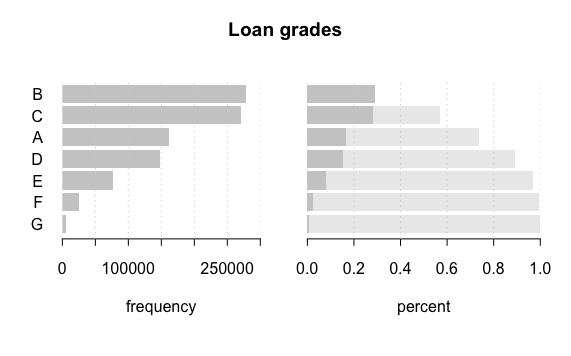
\includegraphics[scale=0.7]{img/grades.png}
	\caption{Kategorie pożyczek.}
	\label{lc:grades}
\end{figure}

Im większe ryzyko inwestycji, tym wyższysz zwrotów oczekują inwestorzy. Znajduje to odzwierciedlenie na wykresie przedstawiającym zależność wysokości stóp procentowych od kategorii pożyczki (Rysunek \ref{lc:int2grade}).

\begin{figure}[h] \centering %H if want to get it exaclty here
	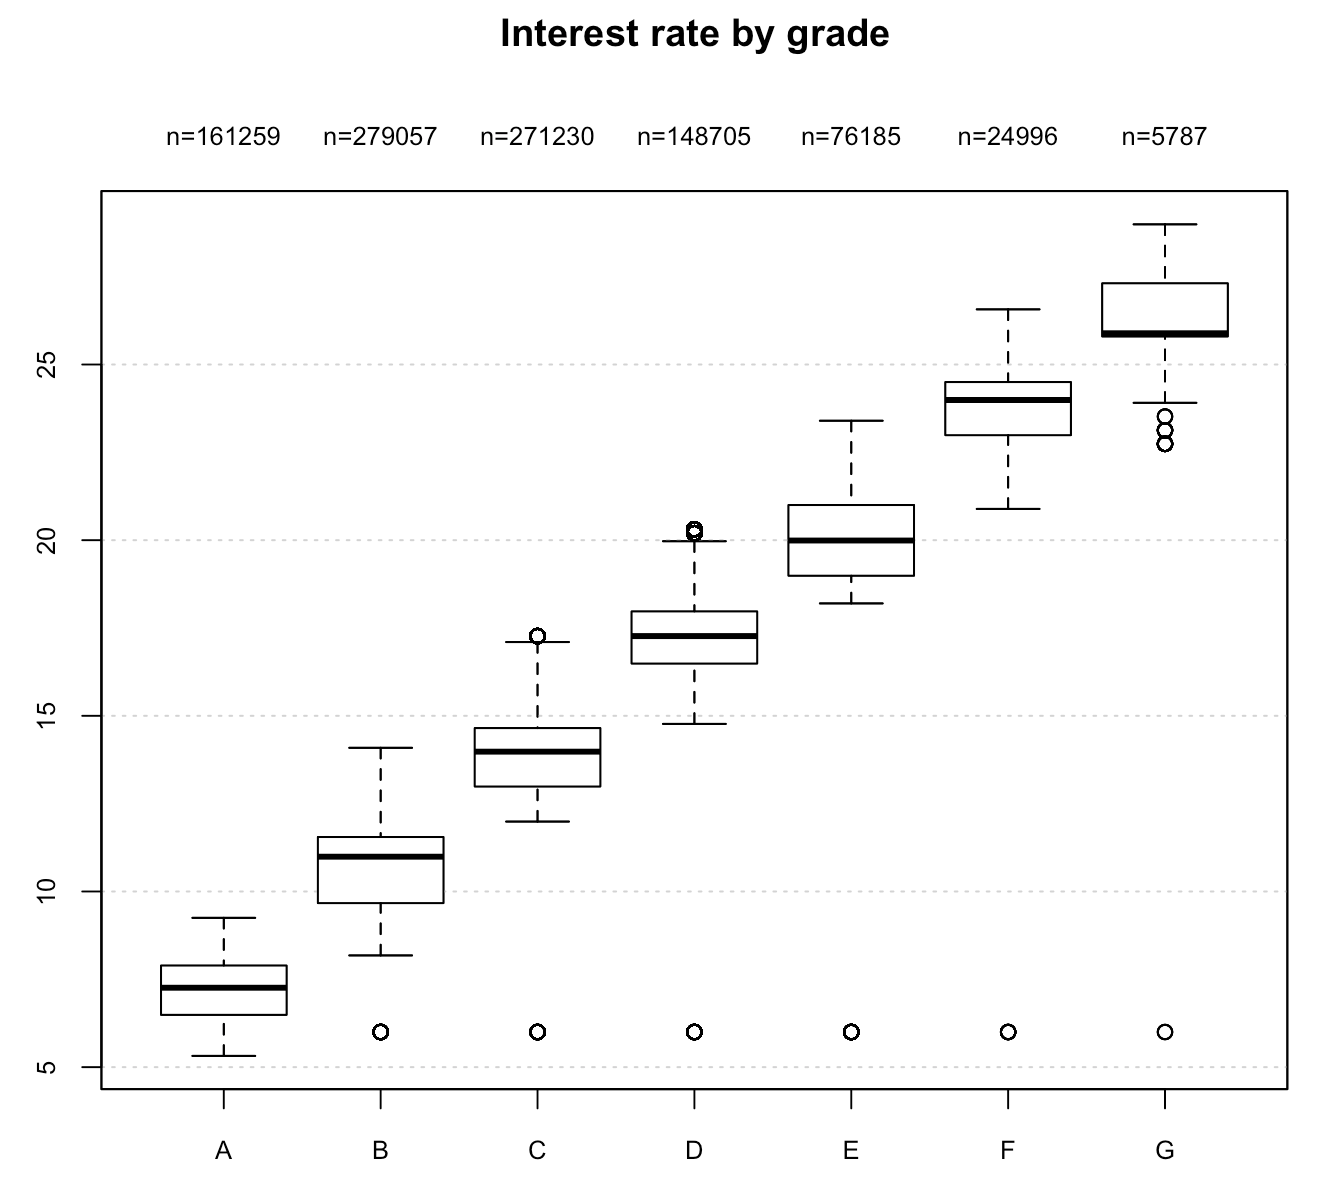
\includegraphics[scale=0.5]{img/int2grade.png}
	\caption{Zależność stóp procentowych od kategorii pożyczki.}
	\label{lc:int2grade}
\end{figure}

\subsection{Statusy pożyczek}

Każda z pożyczek ma przypisany status, który określa jej aktualny stan (Rysunek \ref{lc:statuses}). Najliczniejszymi grupami są bieżące pożyczki (\textit{Current}) i spłacone (\textit{Fully Paid}) - odpowiednio 66\% i 25,3\%, co stanowi 91,3\% wszystkich pozycji. Oznacza to, że 8,7\% pożyczek to pożyczki, które przyniosły straty inwestorom. Jednym z zadań implementowanego systemu będzie wyliczenie prawdopodobieństwa, że bieżąca pożyczka przestanie być spłacana w terminie lub w ogóle nie zostanie zpłacona. Inwestor dzięki tym informacjom będzie mógł aktywnie zarządzać swoim portfolio poprzez wczesną sprzedaż zadłużenia o zbyt dużym ryzyku oraz zakup długów o niskim prawdopodobieństwie niespłacalności. Wykorzystano do tego metodę regresji opartą na modelach uczenia maszynowego, co zostało opisane w następnym rozdziale. W celu przystosowania danych do przeprowadzenia regresji logistycznej, tj. przypadku gdy zmienna zależna przyjmuje tylko dwie wartości \cite{MED}, na etapie wstępnego przetwarzania danych utworzono dodatkową kolumnę \textbf{defaulted}, która przyjmuje wartości \textbf{0} dla pożyczek o pozytywnym lub neutralnym statusie (\textit{Current, Fully Paid, In Grace Period}) oraz \textbf{1} dla tych o negatywnym. Następnie przeprowadzono analizę zależności wartości nowoutworzonej kolumny od atrybutów numerycznych opisujących pożyczkę. Utworzono również dodatkowy atrybut opisujący procentowy stopień spłacenia długu.

\begin{figure}[h] \centering %H if want to get it exaclty here
	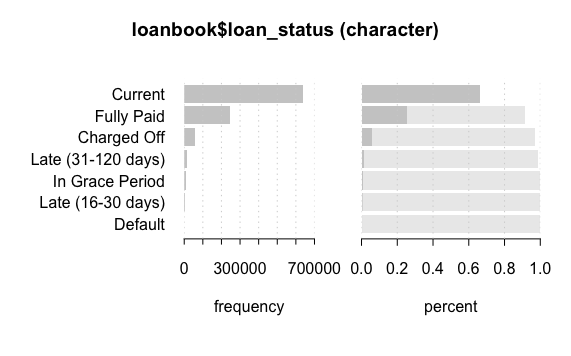
\includegraphics[scale=0.5]{img/statuses.png}
	\caption{Statusy pożyczek.}
	\label{lc:statuses}
\end{figure}

\subsection{Analiza wpływu zmiennych numerycznych na status pożyczki}

Ostatnim etapem analizy danych było zbadanie wpływy poszczególnych atrybutów numerycznych na zachowanie pożyczki. Wykorzystano w tym celu podział na \textit{dobre} i \textit{złe} pożyczki w oparciu o ich statu wprowadzone na etapie wstępnego przetwarzania (utworzenie kolumny \textbf{defaulted} przyjmującej wartości 0 i 1). 

\begin{lstlisting}[language=R, caption={Skrypt wyznaczający macierz koralacji dla zmiennych numerycznych.}, label={r:correlationMatrix}]
set.seed(123)
library(mlbench)
library(caret)

numeric_vars <- sapply(loanbook, is.numeric)
correlationMatrix <- cor(loanbook[, numeric_vars])
correlationMatrix[is.na(correlationMatrix)] <- 0
redundantData <- findCorrelation(correlationMatrix, cutoff = 0.9, verbose = TRUE, names = TRUE, exact = TRUE)
print(correlationMatrix[redundantData, redundantData])
\end{lstlisting}

W celu ograniczenia liczby badanych atrybutów wyznaczono macierz korelacji i usunięto ze zbioru te atrybuty, dla których współczynnik wyniósł ponad 90\% \ref{r:correlationMatrix}.

\begin{figure}[h] \centering %H if want to get it exaclty here
	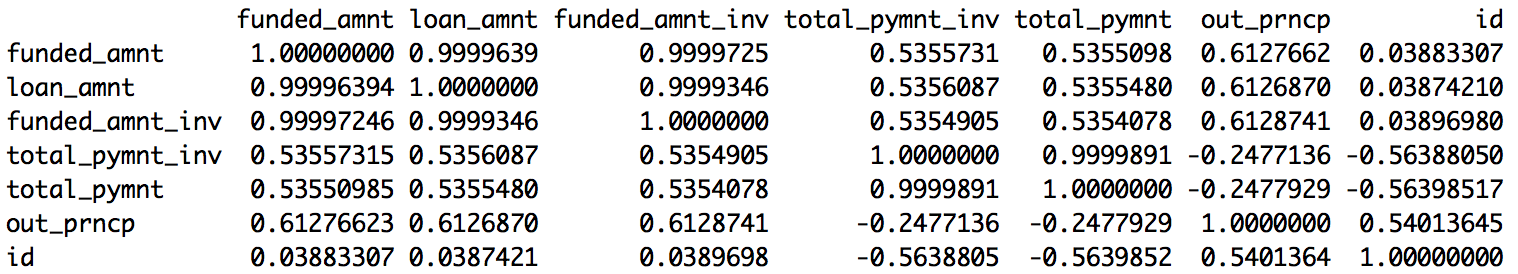
\includegraphics[scale=0.6]{img/redundantData.png}
	\caption{Macierz korelacji dla zmiennych o współczynniku korelacji przekraczającym 90\%.}
	\label{lc:redundantData}
\end{figure}

Na podstawie uzyskanych wyników (Rysunek \ref{lc:redundantData}) wyłączono z dalszej analizy następujące atrybuty:

\begin{itemize}
	\item \textit{funded\_amnt\_inv}, ze względu na korelację z \textit{funded\_amnt},
	\item \textit{total\_pymnt\_inv}, ze względu na korelację z \textit{total\_pymnt},
	\item \textit{funded\_amnt}, ze względu na korelację z \textit{loan\_amnt}.
\end{itemize}
Nie uwzględniano również zmiennej \textit{id}, ponieważ nie ma ona żadnego wpływu na zachowanie długu.

Następnie w oparciu udostępniony słownik danych \cite{LendingClub} wybrano atrybuty, które opisują pożyczkę oraz zdolność kredytową kredytobiorcy:

\begin{itemize}
	\item $loan\_amnt$ - kwota kredytu,
	\item $int\_rate$ - stopa procentowa,
	\item $term$ - okres spłaty kredytu,
	\item $emp\_length$ - okres zatrudnienia kredytobiorcy,
	\item $annual\_inc$ - roczny przychód kredytobiorcy,
	\item $delinq\_2yrs$ - liczba rat, które nie zostały spłacone w terminie w ciągu ostatnich 2 lat,
	\item $dti$ - stosunek zadłużenia do przychodu kredytobiorcy.
\end{itemize}

Ponadto utworzono zmienną $paid\_amount\_ratio$, określającą w jakim stopniu kredyt został już spłacony.

\subsubsection{Zależność pomiędzy wysokością pożyczki, a jej zachowaniem}

\begin{figure}[h] \centering %H if want to get it exaclty here
	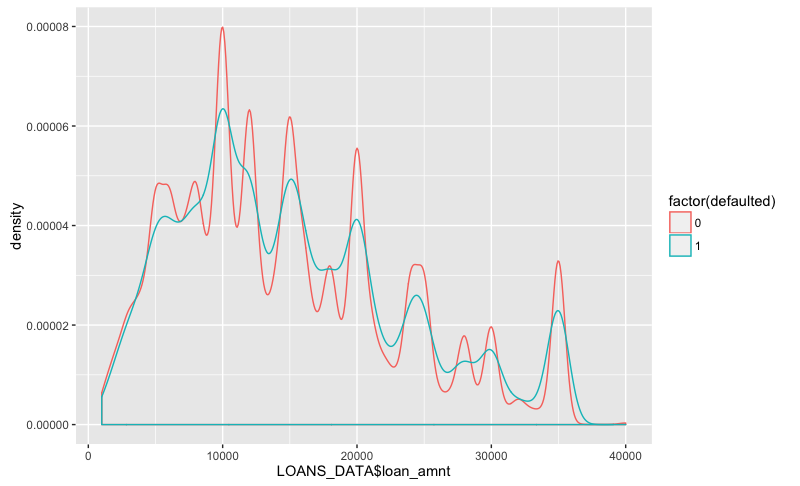
\includegraphics[scale=0.5]{img/amt_defaulted.png}
	\caption{Zależność pomiędzy wysokością pożyczki, a jej zachowaniem.}
	\label{lc:amt_defaulted}
\end{figure}

Wykres przedstawiający tę zależnosć (Rysunek \ref{lc:amt_defaulted}) charakteryzuje się dużą nieregularnością i nie można wydzielić przedziałów wysokości pożyczek, które jednoznacznie wskazywałyby na duże prawdopodobieństwo negatywnego lub pozytywnego zachowania kredytu.

\subsubsection{Zależność pomiędzy wysokością stóp procentowych, a zachowaniem pożyczki}

\begin{figure}[h] \centering %H if want to get it exaclty here
	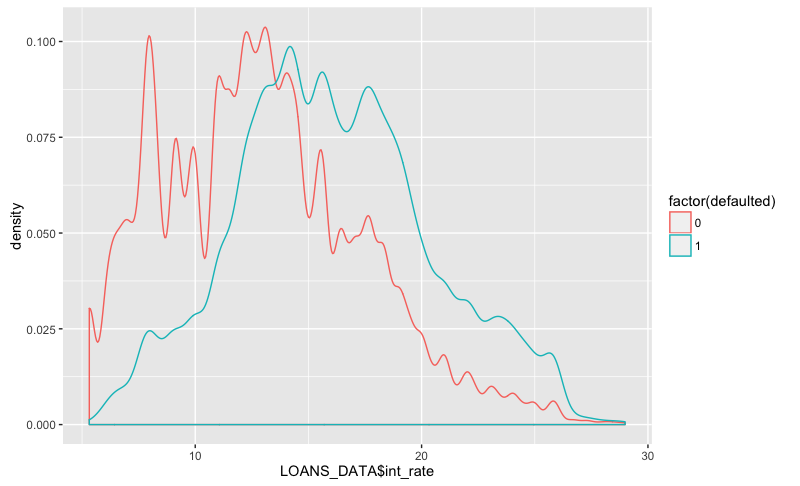
\includegraphics[scale=0.5]{img/int_defaulted.png}
	\caption{Zależność pomiędzy wysokością stóp procentowych, a zachowaniem pożyczki.}
	\label{lc:int_defaulted}
\end{figure}

W tym przypadku zależnosć jest zdecydowanie lepiej widoczna. Na podstawie wykresu (Rysunek \ref{lc:int_defaulted}) można stwierdzić, że prawdopodobieństwo negatywnego zachowania pożyczki znacząco wzrasta wraz z przekroczeniem progu 14\% stopy procentowej. Jest to uzasadnione tym, że wraz ze wzrostem ryzyka wzrasta oczekiwana przez inwestorów stopa zwrotu z inwestycji.

\subsubsection{Zależność pomiędzy okresem, na jaki zawarta jest pożyczka, a jej zachowaniem}

\begin{figure}[H] \centering %H if want to get it exaclty here
	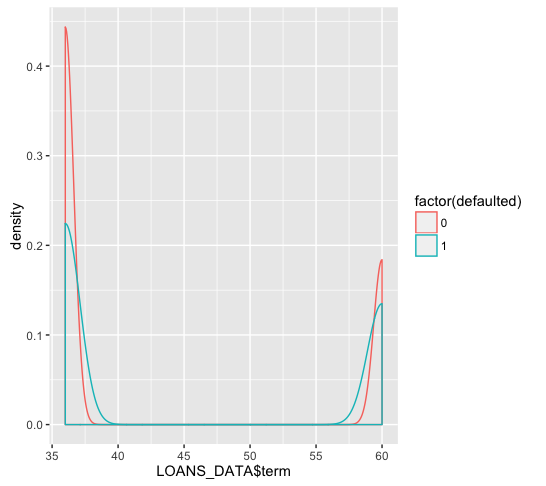
\includegraphics[scale=0.7]{img/term_defaulted.png}
	\caption{Zależność pomiędzy okresem, na jaki zawarta jest pożyczka, a jej zachowaniem.}
	\label{lc:term_defaulted}
\end{figure}

Na podstawie wykresu (Rysunek \ref{lc:term_defaulted}) można jednoznacznie stwierdzić, że dla pożyczek zawartych na krótszy okres czasu ryzyko jest zdecydowanie niższe, niż w przypadku kredytów 5-letnich.

\subsubsection{Zależność pomiędzy długością zatrudnienia kredytobiorcy, a zachowaniem pożyczki}

\begin{figure}[H] \centering %H if want to get it exaclty here
	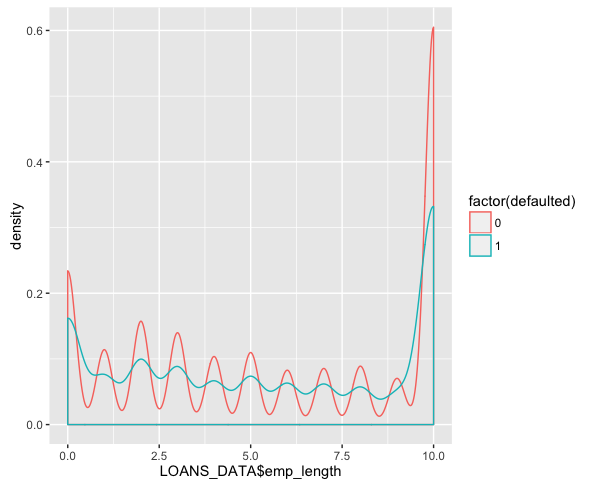
\includegraphics[scale=0.7]{img/emp_defaulted.png}
	\caption{Zależność pomiędzy długością zatrudnienia kredytobiorcy, a zachowaniem pożyczki.}
	\label{lc:emp_defaulted}
\end{figure}

Co zaskakujące, nie ma jednoznacznej zależności pomiędzy długością zatrudnienia kredytobiorcy, a zachowaniem zawieranej przez niego pożyczki (Rysunek \ref{lc:emp_defaulted}). Intuicja sugerowałaby, że wraz ze wzrostem stażu pracy, wzrośnie również stabilność ekonomiczna pożyczkobiorcy, a co za tym idzie spadnie ryzyko negatywnego zachowania pożyczki, jednak obie krzywe są nieregularne.

\subsubsection{Zależność pomiędzy rocznym dochodem kredytobiorcy, a zachowaniem pożyczki}

\begin{figure}[H] \centering %H if want to get it exaclty here
	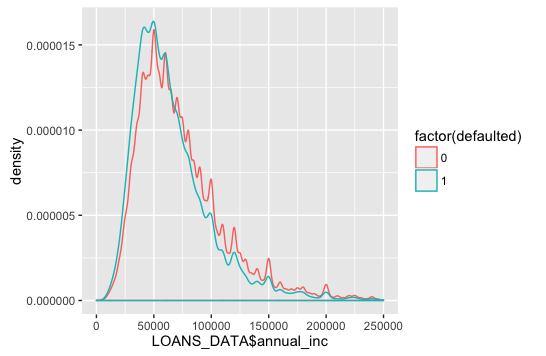
\includegraphics[scale=0.7]{img/inc_defaulted.png}
	\caption{Zależność pomiędzy długością zatrudnienia kredytobiorcy, a zachowaniem pożyczki.}
	\label{lc:inc_defaulted}
\end{figure}

Wysokość rocznego wynagrodzenia nie pozwala określenie prawdopodobnego zachowania pożyczki w zależności przyjętego przedziału dochodu - przebieg obu krzywych jest zbliżony (Rysunek \ref{lc:inc_defaulted}).

\subsubsection{Zależność pomiędzy liczbą spóźnionych rat, a zachowaniem pożyczki}

\begin{figure}[h] \centering %H if want to get it exaclty here
	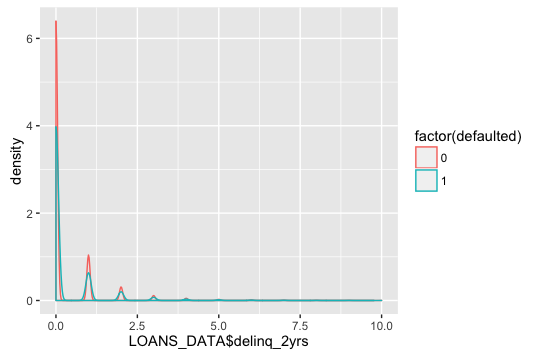
\includegraphics[scale=0.7]{img/delinq_defaulted.png}
	\caption{Zależność pomiędzy liczbą spóźnionych rat, a zachowaniem pożyczki.}
	\label{lc:delinq_defaulted}
\end{figure}

Wykres przedstawiający tę zależność (Rysunek \ref{lc:delinq_defaulted}), wskazuje większe prawdopodobieństwo pozytywnego zachowania pożyczki, jeśli kredytobiorca nigdy nie zalegał ze spłatą rat. W przypadku występowania spóźnionych rat obie krzywe przebiegają w zbliżony sposób.

\subsubsection{Zależność pomiędzy stosunkiem zadłużenia do dochodu kredytobiorcy, a zachowaniem pożyczki}

\begin{figure}[H] \centering %H if want to get it exaclty here
	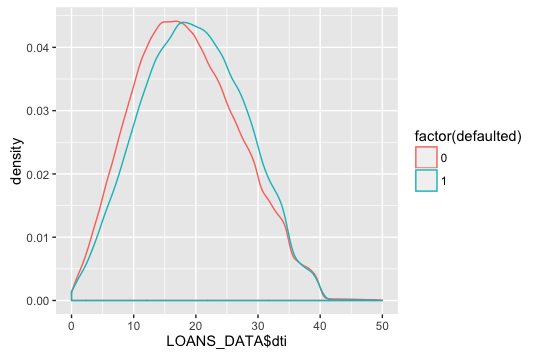
\includegraphics[scale=0.7]{img/dti_defaulted.png}
	\caption{Zależność pomiędzy stosunkiem zadłużenia do dochodu kredytobiorcy, a zachowaniem pożyczki.}
	\label{lc:dti_defaulted}
\end{figure}

Dla wartości zmiennej niższej niż 17\% isnieje większa szansa pozytywnego przebiegu inwestycji, w przypadku wyższych wartości nieznacznie wzrasta ryzyko negatywnego zachowania pożyczki, ale różnice w przebiegu krzywych są niewielkie (Rysunek \ref{lc:dti_defaulted}).

\subsubsection{Zależność pomiędzy stopniem spłaty pożyczki, a jej zachowaniem}

\begin{figure}[H] \centering %H if want to get it exaclty here
	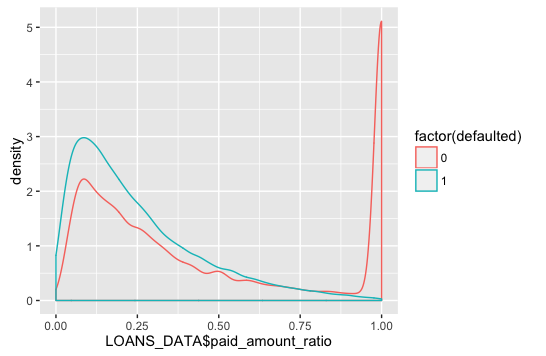
\includegraphics[scale=0.7]{img/paid_defaulted.png}
	\caption{Zależność pomiędzy stopniem spłaty pożyczki, a jej zachowaniem.}
	\label{lc:paid_defaulted}
\end{figure}

Na podstawie tego wykresu (Rysunek \ref{lc:paid_defaulted}), że pożyczki, dla których spłacono przynajmniej 80\% zadłużenia z dużą dozą prawdopodobieństwa zostaną spłacone do końca. Analogicznie dla pożyczek o stopniu spłacenia niższym niż 7\% wzrasta ryzyko niespłacenia pożyczki - oznaczałoby to osoby, które wzięły kredyt z góry zakładając, że nie będą go spłacać. Obie te informacje są cenną wskazówką dla inwestorów, a ponadto pozwalają na określenie przedziałów charakteryzujących się określonym zachowaniem pożyczki, co pozwala zakładać, że ta zmienna powinna zostać wykorzystana w procesie uczenia modelu predykcyjnego.

\subsubsection{Podsumowanie analizy zmiennych numerycznych}

Zmiennymi, od których wartości w największym stopniu zależy zachowanie pożyczki to \textbf{stopień spłaty pożyczki}, \textbf{stopy procentowe} oraz \textbf{okres, na jaki została zawarta pożyczka} - zostaną one wykorzystane przy uczeniu modelu predykcyjnego. Dużym zaskoczeniem jest brak wyraźnej zależności pomiędzy wysokością rocznego dochodu oraz stażem zatrudnienia, a potencjalnym zachowaniem pożyczki.
	\chapter{Model predykcyjny}

\section{Definicja drzewa decyzyjnego}

Ocena ryzyka kredytowego, w tym przypadku predykcja, czy dana pożyczka będzie spłacana zgodnie z obowiązującymi terminami, jest typowym przykładem problemu klasyfikacji wektora danych w oparciu o dane historyczne. W tym celu implementowany system będzie wyposażony w moduł predykcyjny składający się z drzewa decyzyjnego wytrenowanego na wstępnie przetworzonych danych pobranych z serwisu Lending Club.

Drzewo decyzyjne to popularne narzędzie wykorzystywane przy wspomaganiu procesu decyzyjnego, często wykorzystywane w uczeniu maszynowym przy wydobywaniu wiedzy z danych historycznych. Ma ono charakter struktury drzewiastej \cite{MED}, składającej się z:

\begin{itemize}
	\item korzenia, czyli węzła wejściowego drzewa, zawierającego wszystkie dane,
	\item węzłów wewnętrznych zawierających testy na wartościach atrybutów, które określają podzbiór danych spełniających test (z każdego z tych węzłów wychodzi dokładnie tyle gałęzi, ile jest możliwych wyników tego testu),
	\item liści, czyli węzłów, które zawierają informację o klasyfikacji obiektów.
\end{itemize}
Rysunek \ref{tree:example} przedstawia przykładowe drzewo decyzyjne, przedstawiające proces podejmowania decyzji określającej, czy pogoda sprzyja wyjściu z domu, czy nie.

\begin{figure}[H] \centering %H if want to get it exaclty here
	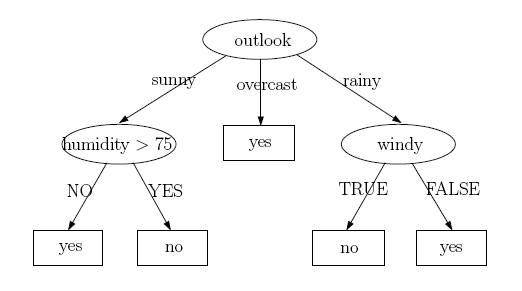
\includegraphics[scale=0.5]{img/decision_tree_example.png}
	\caption{Przykład drzewa decyzyjnego \cite{MED}.}
	\label{tree:example}
\end{figure}

Przy ocenie jakości drzewa należy wziąć pod uwagę następujące cechy \cite{treeMIMUW}:

\begin{itemize}
	\item rozmiar:
		\begin{itemize}
			\item liczba węzłów,
			\item wysokość,
			\item liczba liści,
		\end{itemize}
	\item dokładność klasyfikacji na zbiorze treningowym,
	\item dokładność klasyfikacji na zbiorze testowym.
\end{itemize}
Dobre drzewo decyzyjne charakteryzyje się nie tylko wysoką dokładnością klasyfikacji na zbiorach treningowym i testowym, ale także stosunkowo niewielkim rozmiarem.

\subsection{Konstrukcja drzew decyzyjnych}

Budowa drzewa przebiega w sposób rekurencyjny i składa się z następujących kroków \cite{PJWSTK}:

\begin{enumerate}
	\item Drzewo zaczyna od pojedynczego węzła reprezentującego cały zbiór treningowy.
	\item Jeżeli wszystkie przykłady należą do jednej klasy decyzyjnej, to zbadany węzeł staje się liściem i jest on etykietowany tą decyzją.
	\item W przeciwnym przypadku algorytm wykorzystuje miarę entropii (funkcja przyrostu informacji) jako heurystyki do wyboru atrybutu, który najlepiej dzieli zbiór przykładów treningowych.
	\item Dla każdego wyniku testu tworzy się jedno odgałęzienie i przykłady treningowe są odpowiednio rozdzielone do nowych węzłów (poddrzew).
	\item Algorytm działa dalej w rekurencyjny sposób dla zbiorów przykładów przydzielonych do poddrzew.
	\item Algorytm kończy się, gdy kryterium stopu jest spełnione.
\end{enumerate}
W sytuacji, kiedy dany zbiór składa się z obiektów przypisanych do różnych klas decyzyjnych, eytkietą staje się klasa o najliczniejszej reprezentacji.

Rysunek \ref{tree:algorithm} przedstawia pseudokod algorytmu budowy drzewa decyzyjnego. Kryterium stopu jest spełnione, gdy aktualny zbiór obiektów \cite{treeMIMUW}:

\begin{itemize}
	\item jest pusty,
	\item zawiera obiekty wyłącznie jednej klasy decyzyjnej,
	\item nie ulega podziałowi przez żaden test.
\end{itemize}


\begin{figure}[h] \centering %H if want to get it exaclty here
	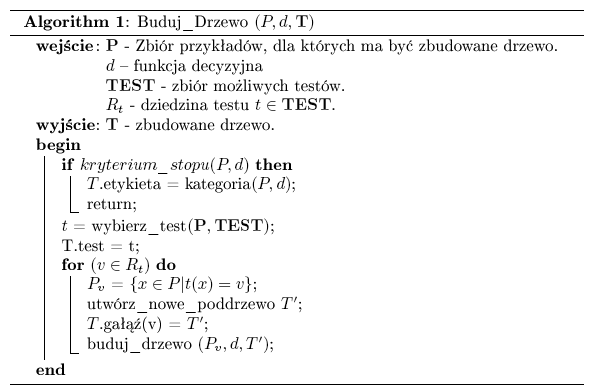
\includegraphics[scale=0.5]{img/tree_algorithm.png}
	\caption{Algorytm budowy drzewa decyzyjnego \cite{PJWSTK}.}
	\label{tree:algorithm}
\end{figure}

\section{Badanie modelu predykcyjnego}

Do budowy modelu predykcyjnego wykorzystano bibliotekę \textbf{party} języka skryptowego \textbf{R}. R jest popularnym narzędziem wykorzystywanym do analizy dużych zbiorów danych i badania pracy algorytmów uczenia maszynowego.

Zadaniem drzewa decyzyjnego będzie klasyfikacja pożyczki do jednej z dwóch klas - 0 lub 1, oznaczających odpowiednio pożyczkę spłaconą w terminie i pożyczkę niespłaconą lub spłaconą po wyznaczonym terminie.

\subsection{Model oparty na wszystkich zmiennych poddanych analizie}

Pierwsze badanie przeprowadzono z wykorzystyniem wszystkich zmiennych numerycznych poddanych analizie w poprzednim rozdziale, tj.:


\begin{itemize}
	\item $loan\_amnt$ - kwota kredytu,
	\item $int\_rate$ - stopa procentowa,
	\item $term$ - okres spłaty kredytu,
	\item $emp\_length$ - okres zatrudnienia kredytobiorcy,
	\item $annual\_inc$ - roczny przychód kredytobiorcy,
	\item $delinq\_2yrs$ - liczba rat, które nie zostały spłacone w terminie w ciągu ostatnich 2 lat,
	\item $dti$ - stosunek zadłużenia do przychodu kredytobiorcy,
	\item $paid\_amount\_ratio$ - stopień, w jakim kredyt został już spłacony.
\end{itemize}

Zgonie z przeprowadzoną analizą, zmiennymi na których powinny oparte być testy wygenerowane przez drzewo powinny być \textbf{int\_rate}, \textbf{term} oraz \textbf{paid\_amount\_ratio}.

W celu wykluczenia danych redundantnych przeprowadzono badanie korelacji pomiędzy poszczególnymi zmiennymi, które wykazało, że nie istnieje pomiędzy nimi zbieżność (Rysunek \ref{tree:correlation}).

\begin{figure}[h] \centering %H if want to get it exaclty here
	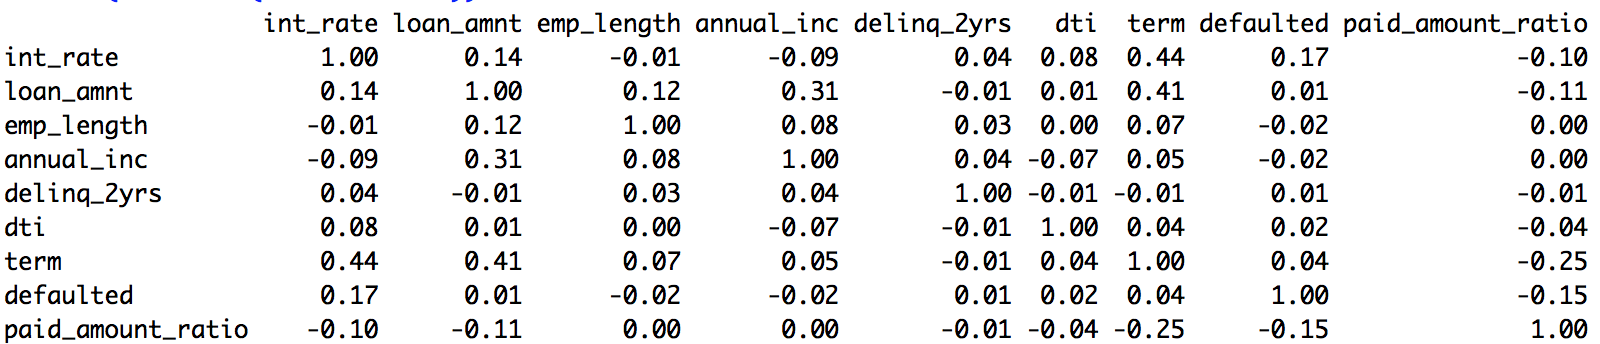
\includegraphics[scale=0.5]{img/tree_correlation.png}
	\caption{Macierz korelacji dla zmiennym wykorzystanych do budowy modelu drzewa decyzyjnego.}
	\label{tree:correlation}
\end{figure}

Następnie przeprowadzono podział zbioru danych na \textbf{treningowy}, \textbf{testowy} i \textbf{walidacyjny} w stosunku 7:2:1.

\begin{sidewaysfigure}
    \centering
    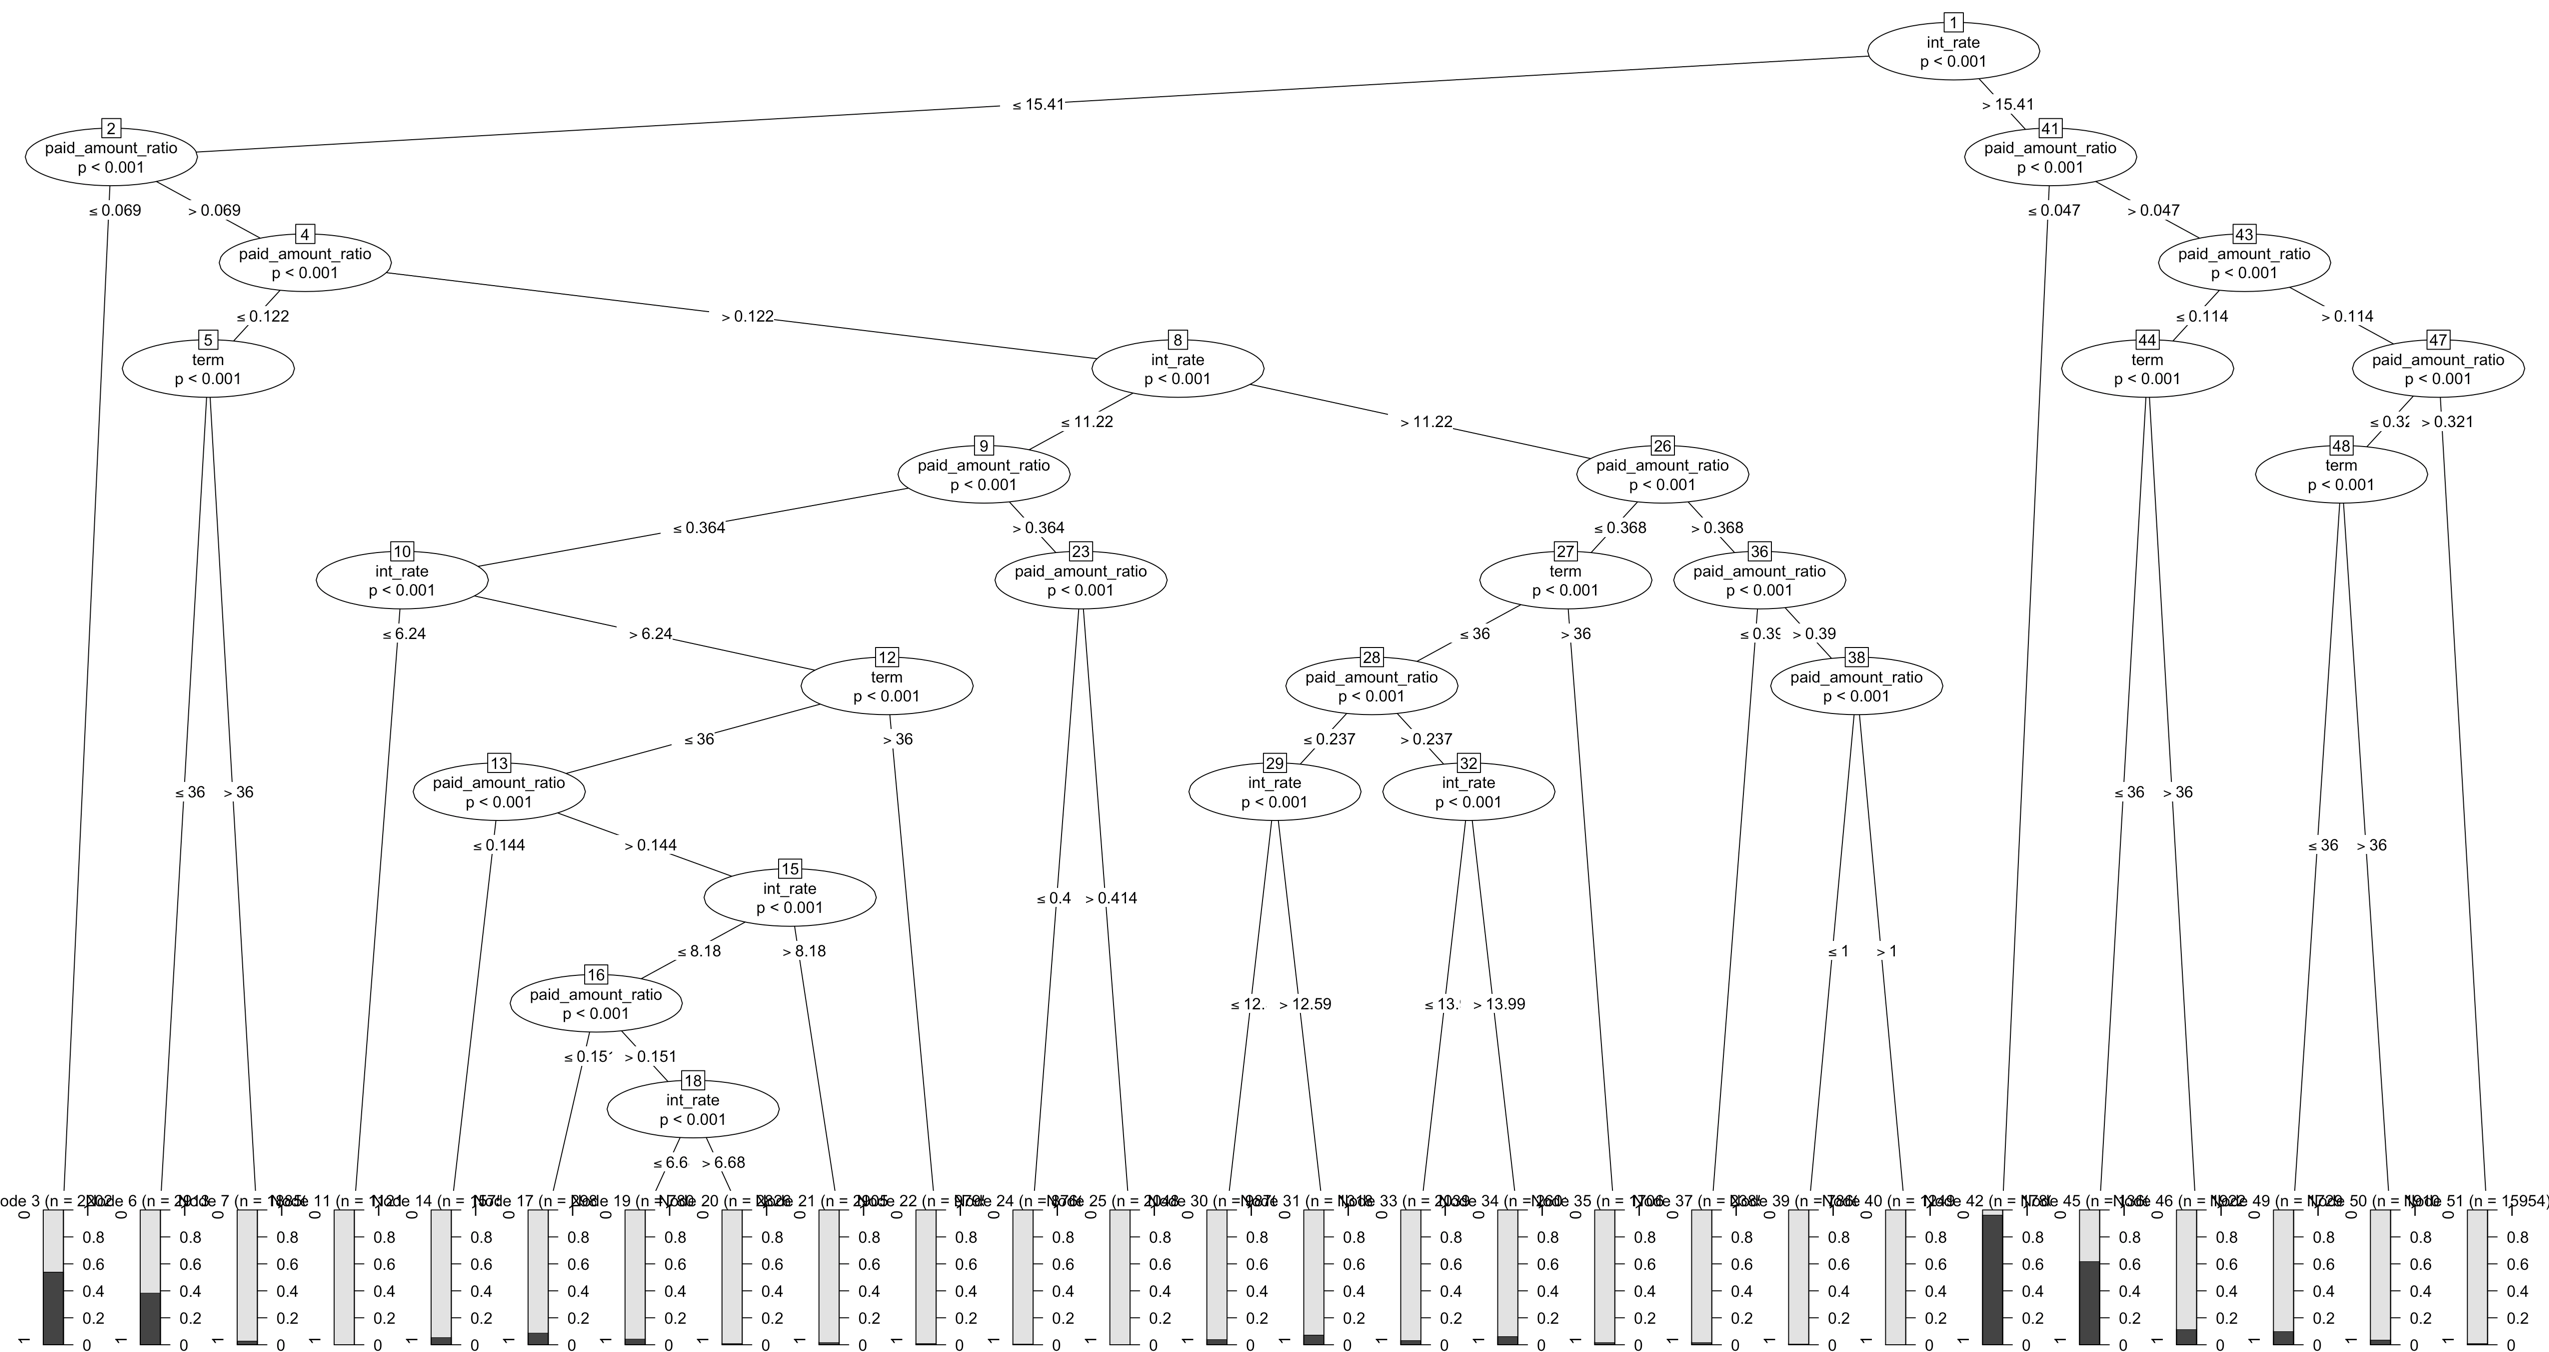
\includegraphics[scale=0.25]{img/tree_full.png}
    \caption{Drzewo decyzyjne uzyskane dla pełnego zakresu zmiennych.}
    \label{tree:full}
\end{sidewaysfigure}

Zgodnie z wynikami przeprowadzonej w poprzednim rozdziale analizy zbioru danych, uzyskany model korzystał jedynie ze zmiennych $int\_rate$, $term$ oraz $paid\_amount\_ratio$ przy tworzeniu kolejnych węzłów (Rysunek \ref{tree:full}) - pozostałe atrybuty mogą zostać pominięte w dalszych badaniach.

Po zbadaniu jakości klasyfikacji na zbiorach testowym i walidacyjnym, uzyskano macierze pomyłek (Tabele \ref{tab:test_full} i \ref{tab:valid_full})wskazujące odpowiednio na 95,04\% i 95,84\% dokładność klasyfikacji, definiowanej jako odsetek poprawnie sklasyfikowanych obiektów.

\begin{table}[h]
\centering 
\setlength\tabcolsep{4pt}
\begin{minipage}{0.48\textwidth}
\centering
\begin{tabular}{|c|r|r|}\hline
\backslashbox{Klasa}{Wynik}
&\makebox[3em]{0}&\makebox[3em]{1}\\\hline\hline

0 & 79545 & 3061 \\ \hline
1 & 498 & 1114 \\	\hline

\end{tabular}
 \caption{Macierz pomyłek dla drzewa decyzyjnego wykorzystującego wszystkie zmienne - zbiór testowy.} 
 \label{tab:test_full}  
\end{minipage}%
\hfill
\begin{minipage}{0.48\textwidth}
\centering
\begin{tabular}{|c|r|r|}\hline
\diagbox{Klasa}{Wynik}
&\makebox[3em]{0}&\makebox[3em]{1}\\\hline\hline

0 & 39802 & 1523 \\ \hline
1 & 228 & 556 \\ \hline

\end{tabular}
 \caption{Macierz pomyłek dla drzewa decyzyjnego wykorzystującego wszystkie zmienne - zbiór walidacyjny.} 
 \label{tab:valid_full} 
\end{minipage}
\end{table}

\subsection{Modele oparte na ograniczonej liczbie zmiennych}

Następnie zbadano modele, w których ogranioczono zbiór zmiennych, które wykorzystano do procesu uczenia. W pierwszej próbie wykorzystano zmienne, które zostały wskazane w wyniku analizy danych przeprowadzonej w poprzednim rozdziale. Uzyskany model (Rysunek \ref{tree:adjusted}) charakteryzuje się mniejszą liczbą węzłów i liści niż poprzedni, oraz większą dokładnością klasyfikacji, na co wskazują uzyskane macierze pomyłek (Tabele \ref{tab:test_adj} i \ref{tab:valid_adj}). Dokładność dla zbioru testowego i walidacyjnego wyniosła odpowiednio 95,66\% i 95,73\%, a liczba węzłów drzewa spadła o 59\% (z 51 do 21) - co z godnie z kryteriami ocenu jakości drzewa decyzyjnego opisanymi na początku tego rozdziału pozwala stwierdzić poprawę jakości modelu.

\begin{sidewaysfigure}
    \centering
    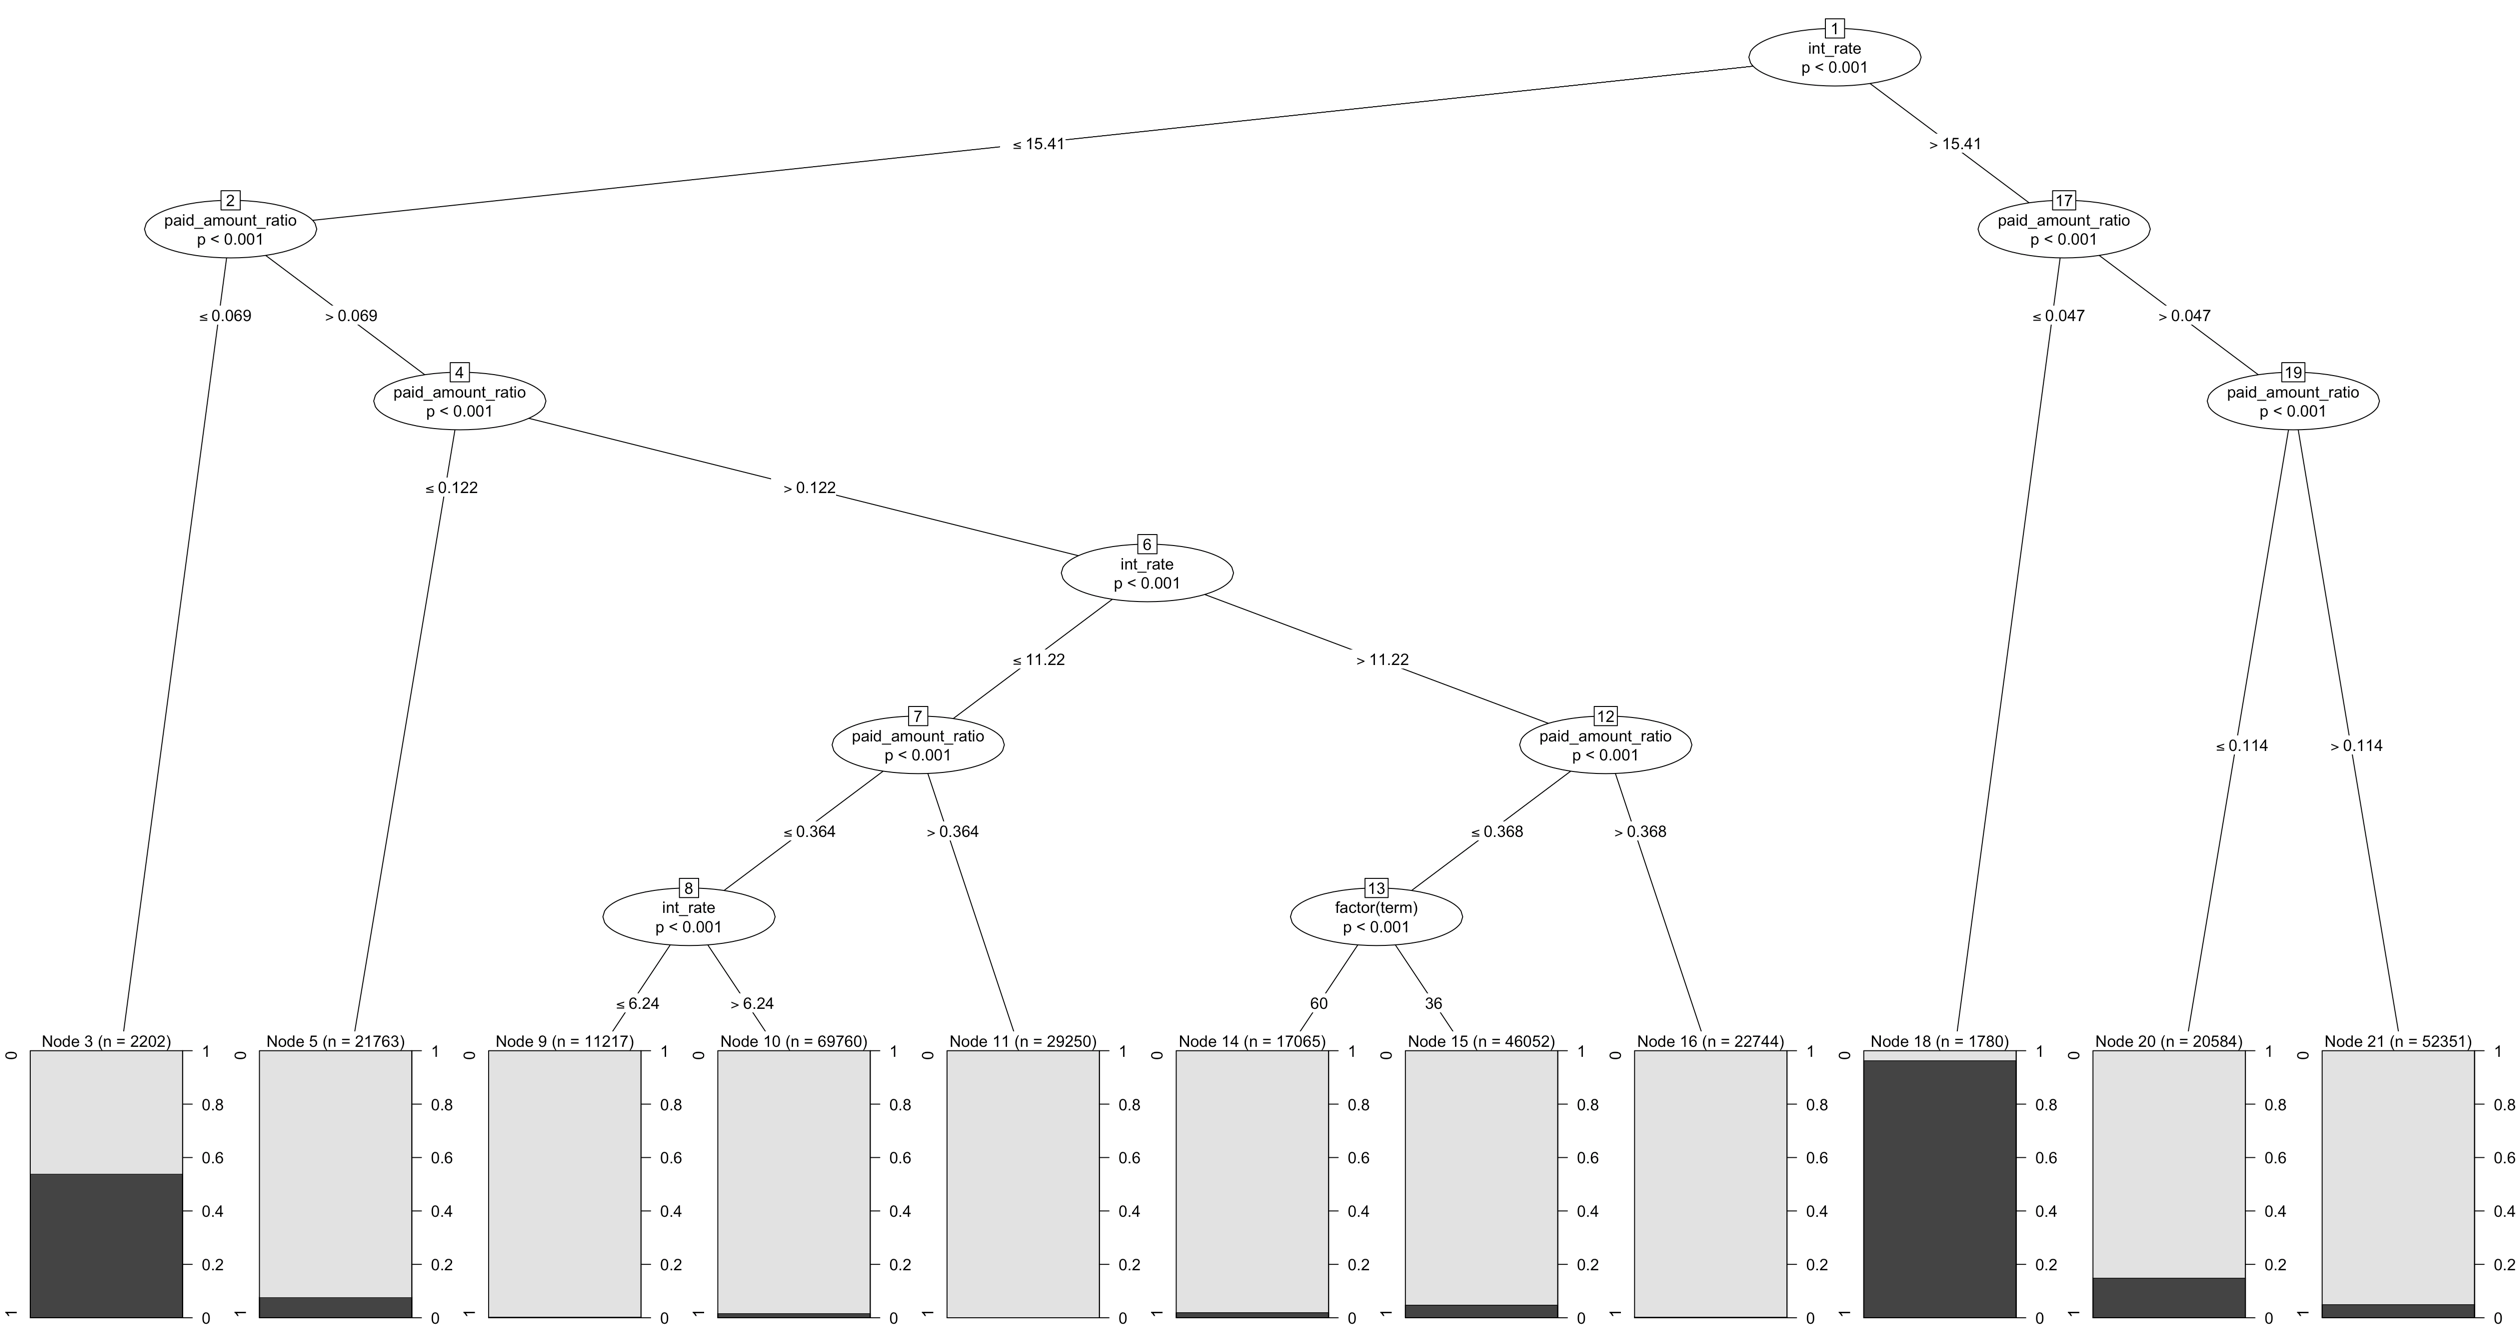
\includegraphics[scale=0.25]{img/tree_adjusted.png}
    \caption{Drzewo decyzyjne uzyskane dla ograniczonego zakresu zmiennych.}
    \label{tree:adjusted}
\end{sidewaysfigure}


\begin{table}[h]
\centering 
\setlength\tabcolsep{4pt}
\begin{minipage}{0.48\textwidth}
\centering
\begin{tabular}{|c|r|r|}\hline
\backslashbox{Klasa}{Wynik}
&\makebox[3em]{0}&\makebox[3em]{1}\\\hline\hline

0 & 79698 & 3306 \\ \hline
1 & 345 & 869 \\	\hline

\end{tabular}
 \caption{Macierz pomyłek dla drzewa decyzyjnego wykorzystującego ograniczony zbiór zmiennych - zbiór testowy.} 
 \label{tab:test_adj}  
\end{minipage}%
\hfill
\begin{minipage}{0.48\textwidth}
\centering
\begin{tabular}{|c|r|r|}\hline
\diagbox{Klasa}{Wynik}
&\makebox[3em]{0}&\makebox[3em]{1}\\\hline\hline

0 & 39882 & 1650 \\ \hline
1 & 148 & 429 \\ \hline

\end{tabular}
 \caption{Macierz pomyłek dla drzewa decyzyjnego wykorzystującego ograniczony zbiór zmiennych - zbiór walidacyjny.} 
 \label{tab:valid_adj} 
\end{minipage}
\end{table}

Ostatnim krokiem przy doborze modelu było sprawdzenie wyników dla poszczególnych par zmiennych. Okazało się, że najlepsze rezultaty uzyskano dla pary zmiennych $paid\_amount\_ratio$ i $term$. Otrzymane drzewo (Rysunek \ref{tree:final}) pozwoliło na redukcję liczby węzłów o 19\% w stosunku do poprzedniego (z 21 do 17) oraz o 67\% w stosunku do pierwotnego drzewa (z 51 do 21). Dokładność klasyfikacji również uległa poprawie - zarówno dla zbioru testowego jak i walidacyjnego wyniosła 95,9\% (Tabele \ref{tab:test_final} i \ref{tab:valid_final})

\begin{sidewaysfigure}
    \centering
    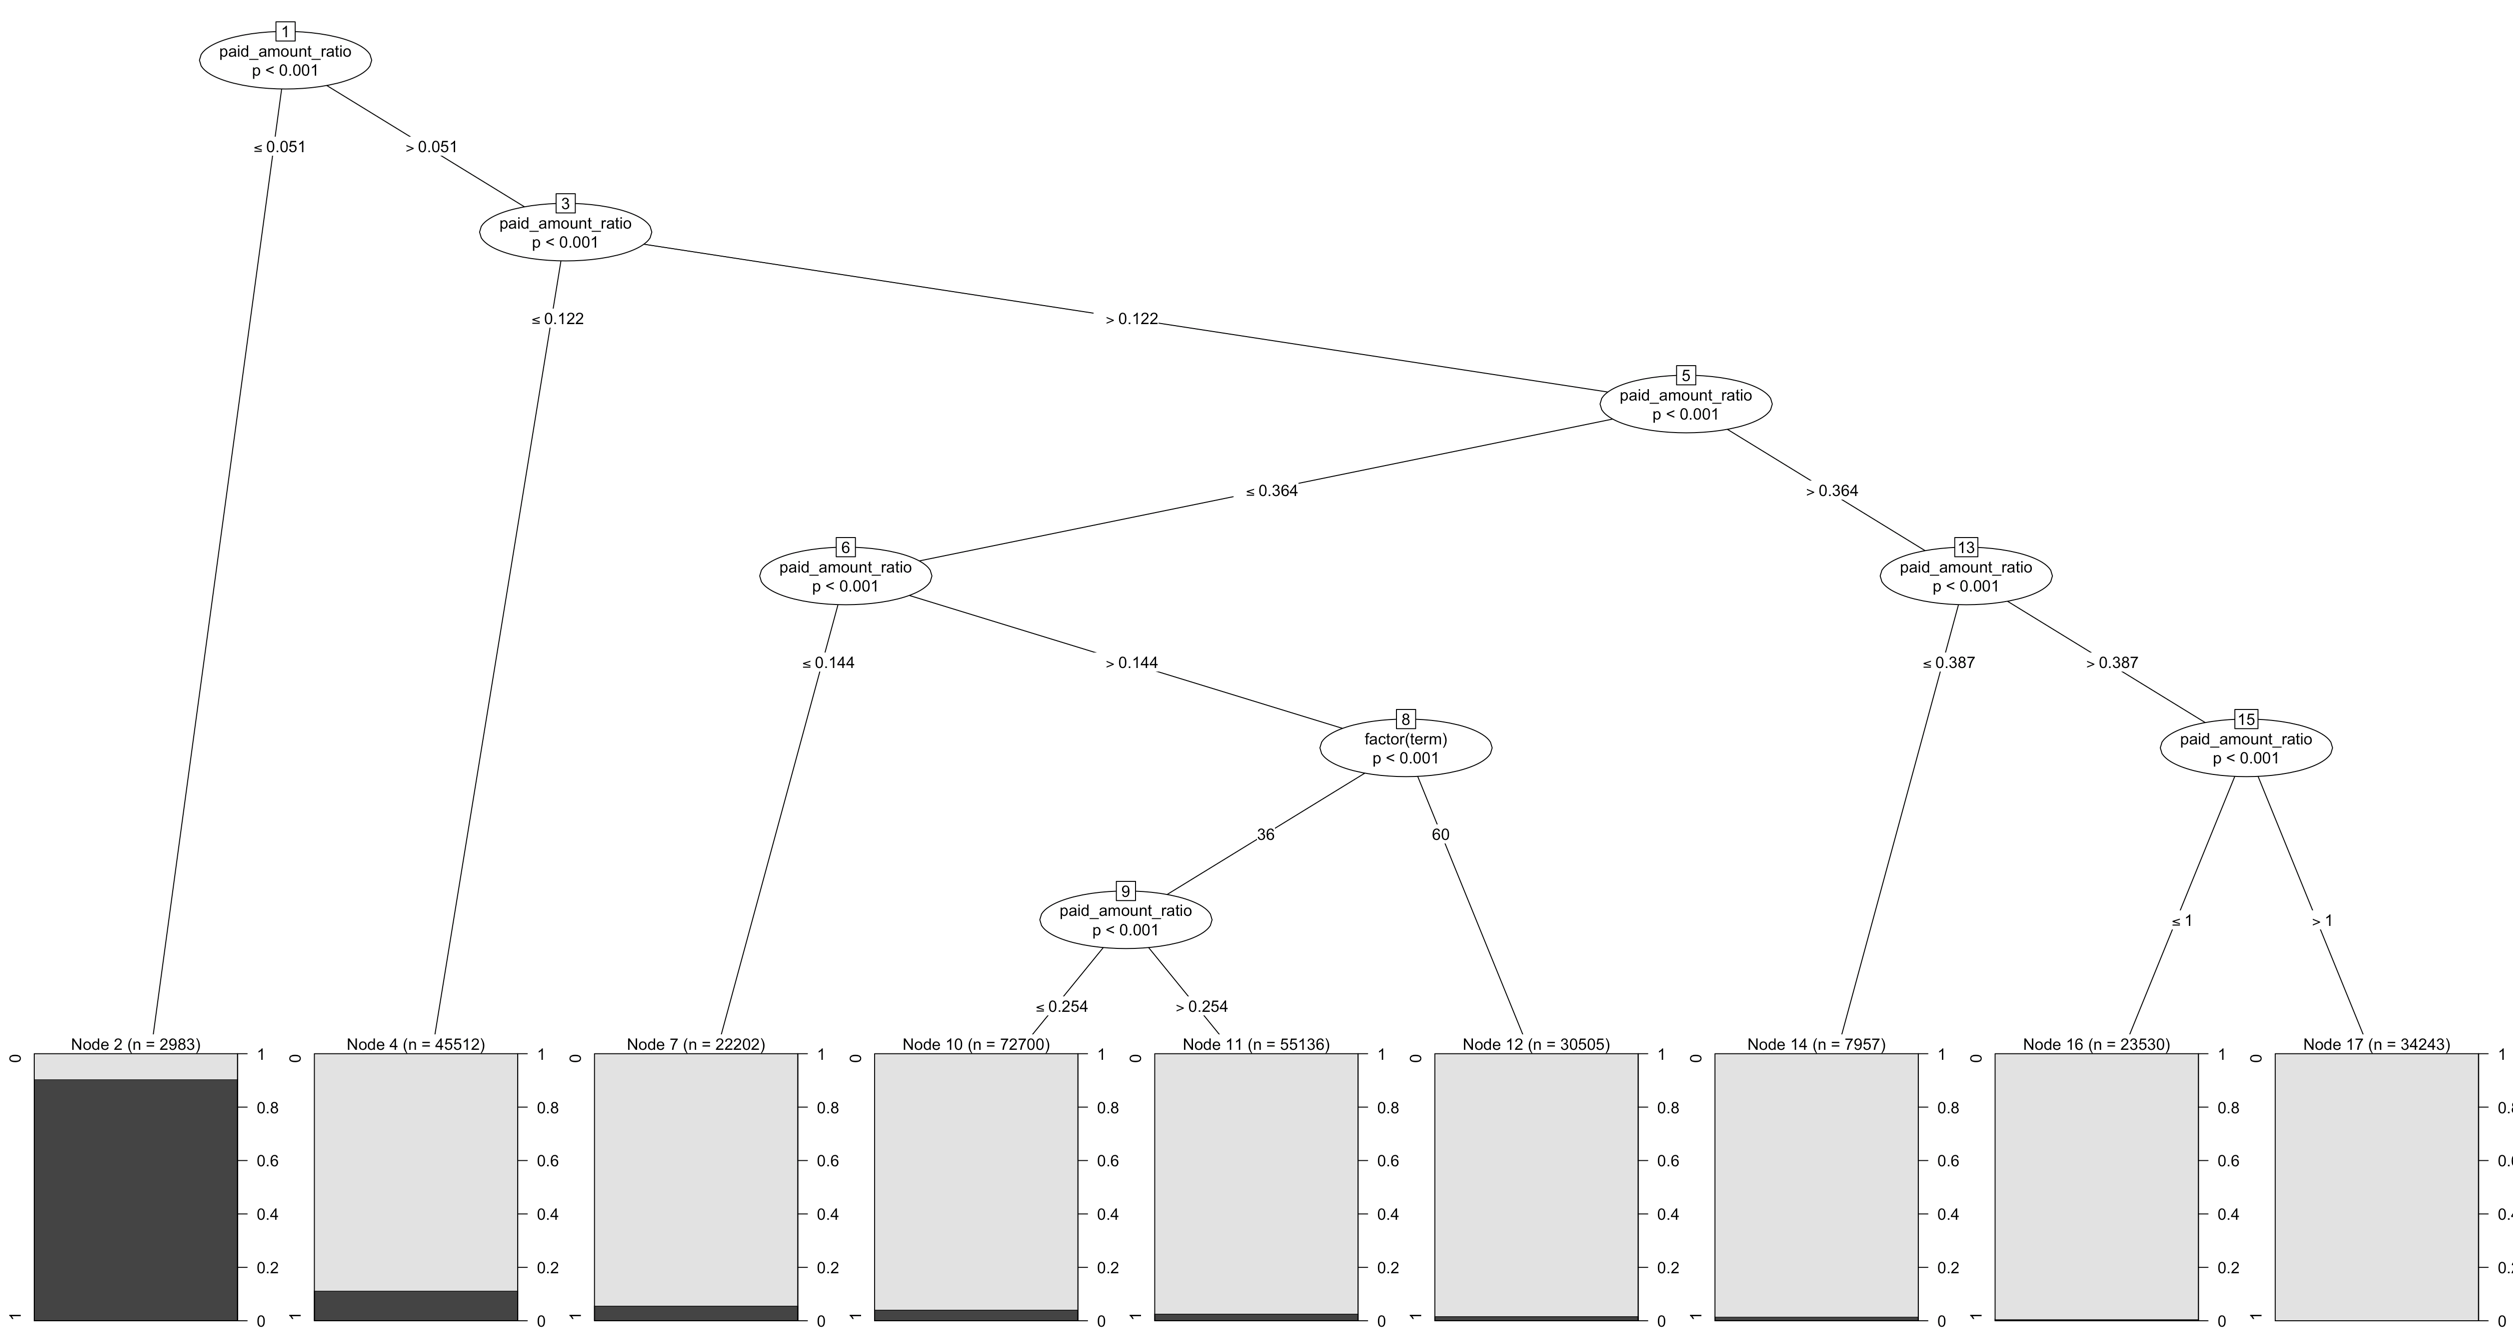
\includegraphics[scale=0.25]{img/tree_final.png}
    \caption{Najlepsze uzyskane drzewo decyzyjne.}
    \label{tree:final}
\end{sidewaysfigure}

\begin{table}[h]
\centering 
\setlength\tabcolsep{4pt}
\begin{minipage}{0.48\textwidth}
\centering
\begin{tabular}{|c|r|r|}\hline
\backslashbox{Klasa}{Wynik}
&\makebox[3em]{0}&\makebox[3em]{1}\\\hline\hline

0 & 79966 & 3372 \\ \hline
1 & 77 & 803 \\	\hline

\end{tabular}
 \caption{Macierz pomyłek dla najlepszego uzyskanego drzewa decyzyjnego - zbiór testowy.} 
 \label{tab:test_final}  
\end{minipage}%
\hfill
\begin{minipage}{0.48\textwidth}
\centering
\begin{tabular}{|c|r|r|}\hline
\diagbox{Klasa}{Wynik}
&\makebox[3em]{0}&\makebox[3em]{1}\\\hline\hline

0 & 39997 & 1683 \\ \hline
1 & 33 & 396 \\ \hline

\end{tabular}
 \caption{Macierz pomyłek dla najlepszego uzyskanego drzewa decyzyjnego - zbiór walidacyjny.} 
 \label{tab:valid_final} 
\end{minipage}
\end{table}

Badania przeprowadzone na drzewach decyzyjnych potwierdzają wyniki analizy przeprowadzonej w poprzednim rozdziale. Okazało się, że zmiennymi które mają wpływ na klasyfikację pożyczek pod względem ich zachowania są $int\_rate$, $term$ oraz $paid\_amount\_ratio$, a szczególnie dwie ostatnie. Ze względu na najwyższą dokładność i jednocześnie najmniejszą liczbę węzłów, w aplikacji zostanie wykorzystany ostatni z badanych modeli.
	\chapter{Aplikacja wspomagająca ocenę ryzyka kredytowego}

\section{Opis aplikacji}

Zadaniem systemu jest dostarczanie inwestorom informacji niezbędnych do podejmowania decyzji o sprzedaży lub kupnie zadłużenia. Użytkownik będzie miał do dyspozycji następujące moduły:

\begin{itemize}
	\item ogólne statystyki pożyczek z podziałem na poszczególne stany USA,
	\item statystyki pożyczek nie spłacanych w terminie,
	\item model predykcyjny, klasyfikujący pożyczki pod kątem ich zachowania (pozytywne lub negatywne).
\end{itemize}

System został zaimplementowany w formie aplikacji webowej, której poszczególne węzły są uruchamiane w konterach aplikacyjnych Docker, co pozwala na uruchomienie w każdym środowisku, w tym chmurze, niezależnie od konfiguracji serwera oraz innych aplikacji, które są na nim uruchomione. Technologia kontenerów aplikacyjnych została szerzej opisana w następnym rozdziale. 

\section{Wykorzystane technologie}

\subsection{AngularJS}

AngularJS jest frameworkiem napisanym w języku JavaScript utrzymywanym przez firmę Google \cite{angular}. Pozwala na realiację wzorca MVC w aplikacji klienciej obsługiwanej przez przeglądarkę internetową, co ułatwia testowanie, utrzymanie oraz rozwój tej części systemu.  Poza realizacją tego wzroca do najważniejszych cech frameworku należą:

\begin{itemize}
	\item dwukierunkowe wiązanie danych (ang. \textit{two-way binding}) - w przeciwieństwie do standardowych systemów szablonowania nie tylko zmiany w warstwie modelu są na bieżąco renderowane w warstwie widoku, ale również zmiany w warstwie widoku wprowadzone przez użytkownika są automatycznie propagowane do warstwy modelu (Rysunek \ref{angular:two_way}. Pozwala to traktować warstwę widoku jako aktualną projekcję modelu.
		\begin{figure}
			\centering
    		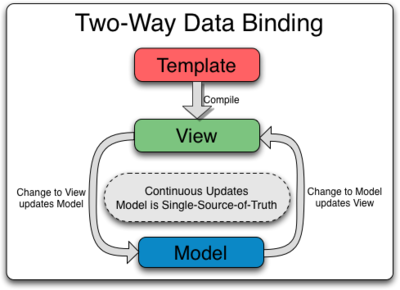
\includegraphics[scale=0.5]{img/Two_Way_Data_Binding.png}
    		\caption{Dwukierunkowe wiązanie danych w AngularJS \cite{angular}.}
    		\label{angular:two_way}
		\end{figure}

	\item odseparowanie logiki aplikacji od maniuplowania strukturą DOM,
	\item odseparowanie warstwy klienckiej od warstwy serwerowej aplikacji webowej,
	\item poprawa testowalności aplikacji klienckiej.
\end{itemize}

\subsection{Node.js}

Node to asynchroniczne, sterowane zdarzeniami środowisko uruchomieniowe języka JavaScript, zaprojektowane z myślą o skalowalnych aplikacjach sieciowych. Prawie żadna z funkcji w Node nie przeprowadza bezpośrednio operacji I/O, co pozwoliło na redykcję ryzyka blokowania procesów \cite{node}.

Node jest zbudowany na podstawie silnika V8 firmy Google, dzięki czemu charakteryzuje się wydajnością prównywalną, a nawet lepszą niż analogiczne aplikacje napisane w języku Java. Zespół pracowników przeprowadził badanie \cite{}
	\chapter{Konteneryzacja aplikacji rozproszonych}

\section{Wyzwania towarzyszące procesowi tworzenia aplikacji rozproszonych}

Wraz z dynamicznym rozwojem Internetu i technologii internetowych pojawiło się zapotrzebowanie na systemy komputerowe będące w stanie wydajnie obsłużyć niebanalne, sięgające dziesiątek, a nawet setek tysięcy, liczby użytkowników oraz jeszcze większe ilości generowanych przez nich zapytań. Idealnym przykładem takich aplikacji są popularne współcześnie portale sieci społecznościowych oraz usługi poczty ele- ktronicznej. Należy przy tym pamiętać, że z punktu widzenia odbiorcy korzystanie z produktu musi dawać poczucie absolutnej transparencji, bez względu na to, jak skomplikowana jest architektura danego rozwiązania. Tworzenie aplikacji będących w stanie spełnić te wymagania wiąże się z szeregiem wyzwań, jakim muszą sprostać deweloperzy. Przedstawiona poniżej lista została opracowana w oparciu o materiał wykładowy przedmiotu „Rozproszone Systemy Operacyjne” prowadzonego przez dr. inż. Tomasza J. Kruka na Wydziale Elektroniki i Technik Informacyjnych Politechniki Warszawskiej \cite{RSO}.

\subsection{Skalowalność}

Wstępny etap projektowania rozwiązania musi obowiązkowo obejmować analizę skalowalności danego rozwiązania. W oparciu o przyjęte założenia systemu, zespół projektowy szacuje liczbę użytkowników danego serwisu, a następnie bazując na tych danych inżynierowie pracujący nad danym rozwiązaniem wyliczają przybliżony ruch sieciowy oraz zasoby niezbędne do płynnego i wydajnego działania systemu. Ponadto przeprowadzenie analizy skalowalności aplikacji rozproszonej na etapie jej projektowania ułatwia identyfikację tzw. „wąskich gardeł”, które mogą w przyszłości ograniczyć, bądź wręcz uniemożliwić rozwój aplikacji.

\subsection{Obsługa różnych języków programowania oraz narzędzi deweloperskich}

Cechą charakterystyczną aplikacji webowych jest pluralizm wykorzystywanych technologii. Dotyczy on zarówno doboru stosowanych bibliotek w obrębie danej technologii, jak również płaszczyzny wyboru języka programowania. Poszczególne moduły mogą być rozwijane przez niezależne zespoły, pracujące w zupełnie odmiennych środowiskach technologicznych. Niesie to za sobą ryzyko konfliktów, które mogą wystąpić przy próbie integracji komponentów. Problemy tego typu są bardzo trudne do przewidzenia na etapie planowania harmonogramu projektu, przez co mogą mieć zasadniczy wpływ na ewentualne przekroczenie pierwotnie zakładanych terminów, co bardzo często wiąże się z karami finansowymi.

\subsection{Długotrwały proces tworzenia środowisk deweloperskich oraz testowych}

W przypadku tworzenia rozległych systemów mamy do czynienia z wieloma środowiskami, które są wykorzystywane do rozwijania oraz testowania produktu na kolejnych etapach pracy. Weryfikacji mogą podlegać między innymi takie cechy aplikacji, jak wydajność, bezpieczeństwo oraz ergonomia, a ponieważ każdy z tych testów często wymaga innej konfiguracji, wiąże się to z koniecznością przygotowania i utrzymywania stosownych przestrzeni testowych. Najpopularniejsze rodzaje środowisk, wykorzystywanych w poszczególnych fazach rozwoju aplikacji, to: wspomniane już środowisko testowe, deweloperskie oraz produkcyjne. Z punktu widzenia zarządzania cyklem życia projektu, każde z nich powinno być wyizolowane i niezależne od pozostałych. Ponadto konfiguracja powinna być łatwa do zarządzania i spójna, tak aby było możliwe odtworzenie danego typu środowiska w każdych warunkach. Szczególnie interesującym i wymagającym przypadkiem jest przygotowanie aplikacji do testów. Bardzo często wiąże się to z konfiguracją nie tylko samej aplikacji, ale również komponentów zewnętrznych, od których jest zależna, np. baz danych. Sytuacja, w której chcemy udostępnić bazę danych wraz z wygenerowanymi na potrzeby testów danymi (które następnie mogą być modyfikowane) wielu deweloperom pracującym nad różnymi aplikacjami jest idealnym przykładem zastosowania kontenerów, które zostaną opisane w dalszej części artykułu.tywanych w poszczególnych fazach rozwoju aplikacji, to: wspomniane już środowisko testowe, deweloperskie oraz produkcyjne. Z punktu widzenia zarządzania cyklem życia projektu, każde z nich powinno być wyizolowane i niezależne od pozostałych. Ponadto konfiguracja powinna być łatwa do zarządzania i spójna, tak aby było możliwe odtworzenie danego typu środowiska w każdych warunkach. Szczególnie interesującym i wymagającym przypadkiem jest przygotowanie aplikacji do testów. Bardzo często wiąże się to z konfiguracją nie tylko samej aplikacji, ale również komponentów zewnętrznych, od których jest zależna, np. baz danych. Sytuacja, w której chcemy udostępnić bazę danych wraz z wygenerowanymi na potrzeby testów danymi (które następnie mogą być modyfikowane) wielu deweloperom pracującym nad różnymi aplikacjami jest idealnym przykładem zastosowania kontenerów, które zostaną szerzej opisane w dalszej części rozdziału.

\subsection{Relatywnie niska wydajność dostarczania rozwiązań na środowisko produkcyjne}

Ze względu na skomplikowany proces wdrażania aplikacji do użytku, szczególnie w przypadku systemów korporacyjnych, gdzie zachodzi konieczność certyfikacji poszczególnych rewizji produktu, efektywność często pozostawia wiele do życzenia. Warto zwrócić uwagę na to, że usprawnienie poszczególnych etapów (np. fazy testowania aplikacji, przytoczonej w poprzednim paragrafie), pozwoli na skrócenie całego cyklu rozwoju aplikacji.

\subsection{Niespójność środowisk}

Problem ten jest szczególnie widoczny podczas wdrażania nowego dewelopera do projektu, kiedy ryzyko występowania różnic pomiędzy poszczególnymi środowiskami jest największe. Podczas konfiguracji stanowiska pracy, nowi pracownicy mogą popełnić błąd, np. instalując złą wersję danego narzędzia, który może następnie wywoływać nieprzewidziane konflikty. Często prowadzi to do dobrze znanej sytuacji, kiedy aplikacja poprawnie działa w obrębie jednego środowiska i sprawia nieoczekiwane problemy w przypadku innych konfiguracji.

\subsection{Bezpieczeństwo aplikacji}

 Ze względu na zasięg, rozmiar i stopień skomplikowania, aplikacje rozproszone są bardziej narażone na ataki ze strony osób niepożądanych. W trakcie wykładu z „Rozproszonych Systemów Operacyjnych” dr Kruk wielokrotnie zwracał uwagę na to, że jest to niestety najczęściej niedoinwestowany aspekt projektów informatycznych, który może mieć znaczący wpływ na bezpieczeństwo użytkowników aplikacji (np. ochronę ich danych osobowych).

 \subsection{Wydajność uruchamiania, wyłączania oraz zarządzania kolejnymi instancjami aplikacji oraz zapewnianie jej dostępności}

 To zagadnienie szczególnie zyskało na znaczeniu wraz z rozwojem usług hostingu dostarczanych w chmurze. Architektura usług oferowanych przez poszczególnych dostawców różni się, przez co pojawiło się zapotrzebowanie na narzędzia, które pozwoliłyby zautomatyzować proces konfiguracji oraz zarządzania życiem aplikacji w chmurze. Niektóre firmy (np. DigitalOcean, AWS) wspierają uruchamianie aplikacji umieszczonych w kontenerach. Wykorzystanie tej technologii pozwala na szybkie uruchamianie kolejnych instancji aplikacji, dzięki czemu łatwiej jest zapewnić jej dostępność na wymaganym przez klienta poziomie.

 \section{Narzędzia do zarządzania konfiguracją środowiska i infrastrukturą aplikacji}

W odpowiedzi na wzrastające zapotrzebowanie powstały narzędzia, które odciążyły deweloperów w zakresie zarządzania grupą identycznych serwerów, uruchamiających te same aplikacje i udostępniających te same usługi.

\begin{figure}[h] \centering %H if want to get it exaclty here
	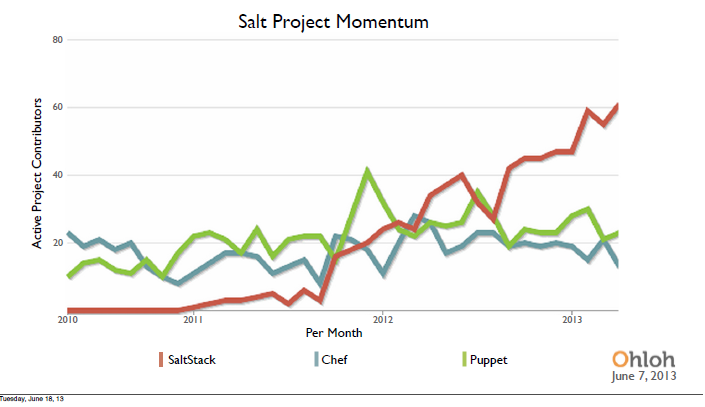
\includegraphics[scale=0.4]{img/salt.png}
	\caption{Porównanie dynamiki rozwoju narzędzi SaltStack, Chef i Puppet na przestrzeni lat 2010-2013\cite{virtualization}}
	\label{salt:chart}
\end{figure}

Jednym z najbardziej dynamicznie rozwijanych rozwiązań (Rysunek \ref{salt:chart}) na rynku jest SaltStack Enterprise\cite{saltstack}. Pozwala ono na sprawne zarządzanie infrastrukturą aplikacji oraz efektywne dostarczanie nowych komponentów do środowiska produkcyjnego. Poza zarządzaniem tradycyjnymi serwerami, SaltStack umożliwa integrację z chmurą i utworzenie abstrakcyjnej, łatwo zarządzalnej warstwy infrastruktury, którą można elastycznie dostosować do różnych aplikacji.
Konkurencyjnym rozwiązaniem, które oferuje automatyzację zarządzania konfiguracją jest Puppet \cite{puppet} występujący w wersji darmowej (Open Source) oraz komercyjnej (Enterprise).

W zestawieniu (Tabela \ref{table:salt}) występują dwa kolejne produkty: Chef oraz Ansible. Opracowanie to zostało przygotowane przez redakcję strony Infoworld, w celu porównania narzędzi wspomagających zarządzanie infrastrukturą aplikacji rozproszonych. Poszczególne produkty zostały ocenione w 10-cio stopniowej skali. Przedstawione kategorie dotyczą zarządzania infrastrukturą aplikacji, ale w dużej mierze pokrywają się z zagadnieniami omówionymi w poprzedniej sekcji (zostały rozszerzone o „Interoperacyjność” oraz „Cena/jakość”). 

\newcommand*\rot{\rotatebox{90}}

\begin{table}[h]
\centering 
\caption{Porównanie narzędzi wspomagających zarządzanie infrastukturą aplikacji \cite{infoworld}}
\label{table:salt}
	\begin{tabular}{@{} cl*{7}c @{}}
		& & \multicolumn{7}{c}{Kategoria oceny i jej waga} \\[2ex]
        & & \rot{Skalowalność (20\%)} & \rot{Dostępność (20\%)} & \rot{Wydajność (20\%)} & \rot{Cena/Jakość (10\%)} 
        & \rot{Zarządzanie usługą (20\%)} & \rot{Interoperacyjność (20\%)}& \rot{Ocena końcowa (100\%)}\\
   		\cmidrule[1px]{2-9}
   		& AnsibleWorks Ansible 1.3 & 8.0 & 9.0 & 9.0 & 9.0 & 8.0 & 7.0 & 8.2 \\
   		& Enterprise Chef 11.4 & 9.0 & 9.0 & 8.0 & 9.0 & 7.0 & 8.0 & 8.3 \\
   		& Puppet Enterprise 3.0 & 9.0 & 9.0 & 9.0 & 9.0 & 9.0 & 9.0 & 9.0 \\
   		\rot{\rlap{~Produkt}}
   		& SaltStack Enterprise 0.17.0 & 9.0 & 9.0 & 9.0 & 9.0 & 9.0 & 8.0 & 8.8 \\
        \cmidrule[1px]{2-9} 
	\end{tabular}
\end{table}

Wszystkie wymienione rozwiązania dostarczają podobnej funkcjonalności, przy czym należy zwrócić uwagę na to, że SaltStack i Ansible to elastyczne i dynamicznie rozwijające się produkty, które stosunkowo niedawno weszły na rynek. Pozostałe dwie pozycje z zestawienia, to bardziej dojrzałe rozwiązania, skierowane przede wszystkim do użytkowników korporacyjnych. Wynika z tego wyższe, w przypadku SaltStack i Ansible, ryzyko znaczących aktualizacji, które mogą mogą wymusić zmiany w projekcie, co sprawia, że te produkty są odpowiednie dla bardziej elastycznych klientów.

\section{Narzędzia do tworzenia wyizolowanych środowisk}

Ta grupa narzędzi koncentruje się na tworzeniu wyizolowanych środowisk deweloperskich w oparciu o instrukcje zapisane w pliku konfiguracyjnym. Popularnym narzędziem tego typu jest Vagrant\cite{vagrant}. Idea tego produktu opiera się na rzeniu maszyny wirtualnej, w której następnie osadzane jest prekonfigurowane środowisko. Kolejne kroki procedury tworzenia tego środowiska są opisane w pliku, który zgodnie z wymogami narzędzia musi nosić nazwę „Vagrantfile”. Niestety, wykorzystanie maszyn wirtualnych wiąże się z narzutem wydajnościowym, a także uzależnia dewelopera od zewnętrznego dostawcy technologii VM (w przypadku Vagrant’a jest to VMWare \cite{vagrant}).

\section{Kontenery aplikacyjne}

Idea kontenerów polena na tworzeniu ``opakowań'' dla aplikacji, które przechowują:

\begin{itemize}
\item kod programu,
\item run time,
\item narzędzia systemowe,
\item biblioteki,
\end{itemize}
niezbędne do poprawnego działania systemu. Jest to ewolucja w stosunku do narzędzi typu Vagrant – kontenery współdzielą ze sobą jądro systemu operacyjnego oraz jego zasoby, natomiast zapewniają izolację na poziomie procesów. Warto zwrócić uwagę na fakt, że jest to technologia oparta na otwartych standardach platformy Linux, na której koncepcja izolacji procesów i ich środowiska jest obecna już od jakiegoś czasu. Kontenery mają za zadanie przede wszystkim zapewnić izolację aplikacji oraz spójność jej środowiska. Adresuje to przytaczane wcześniej problemy, z którymi muszą się mierzyć deweloperzy aplikacji rozproszonych, z naciskiem na redukcję ryzyka wystąpienia konfliktu pomiędzy wykorzystanymi technologiami, braku koherencji środowisk: deweloperskiego, testowego i produkcyjnego, a także trudności z wdrażaniem nowych deweloperów do projektu.

\subsection{Kontenery a maszyny wirtualne}

Główny mechanizm obu rozwiązań jest bliźniaczo podobny (\ref{fig:vm2docker}) – różnica w przypadku kontenerów polega na współdzieleniu przez nie jądra systemu operacyjnego i jego zasobów, dzięki czemu udało się ograniczyć znaczny narzut wydajnościowy jakim obarczone są maszyny wirtualne \cite{infoworld, vagrant, docker}.

\begin{figure}[h]
\centering
\begin{subfigure}{.5\textwidth}
  \centering
  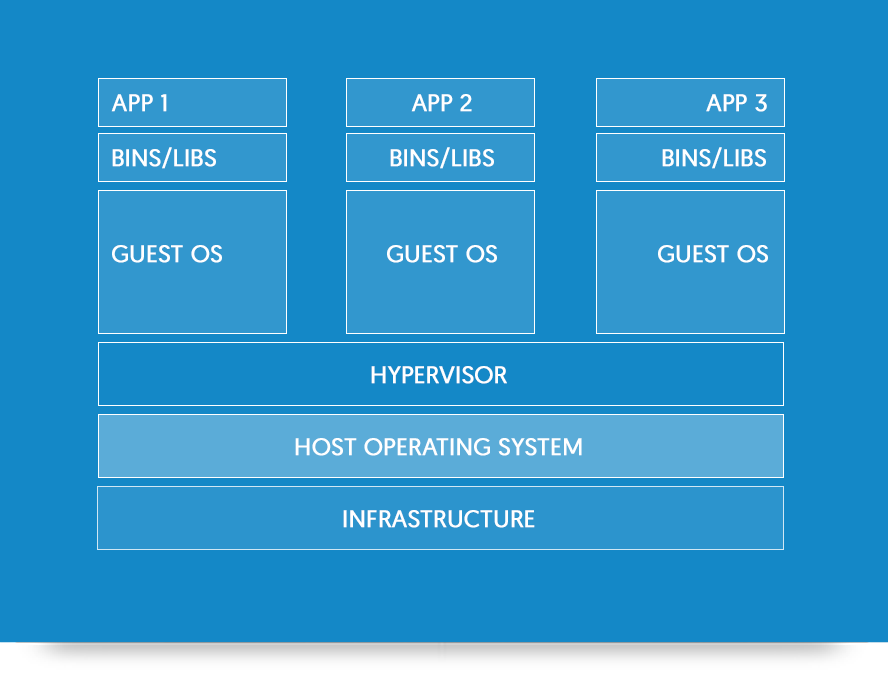
\includegraphics[width=.8\linewidth]{img/vm.png}
  \caption{Architektura maszyny wirtualnej}
  \label{fig:vm}
\end{subfigure}%
\begin{subfigure}{.5\textwidth}
  \centering
  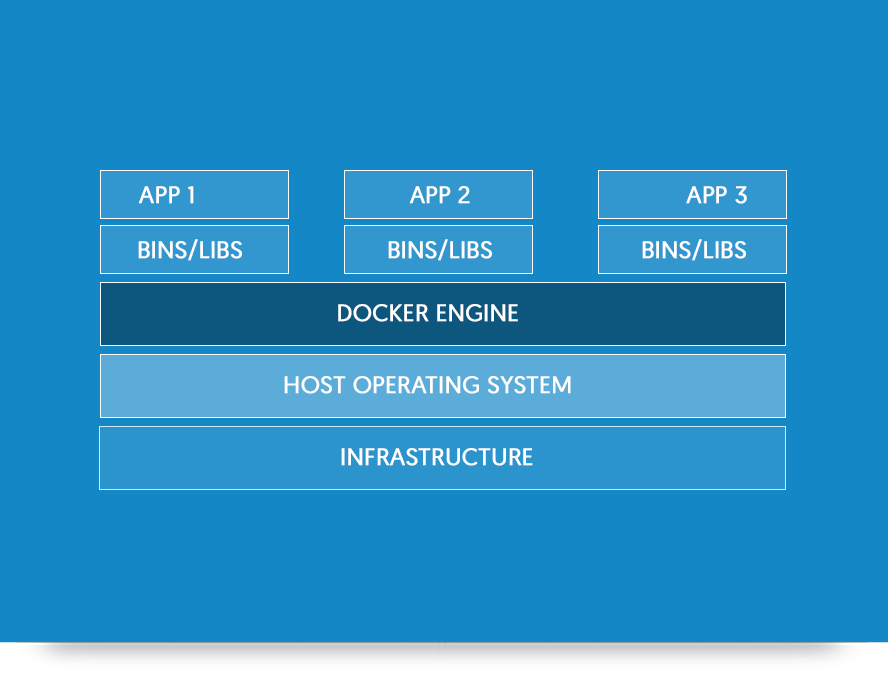
\includegraphics[width=.8\linewidth]{img/docker.png}
  \caption{Architektura kontenera}
  \label{fig:docker}
\end{subfigure}
\caption{Porównanie architetury maszyny wirtualnej i kontenera}
\label{fig:vm2docker}
\end{figure}

\begin{table}[h]
\centering 
\caption{Porównanie kontenerów i maszyn wirtualnych na przykładzie Dockera i Vagranta \cite{docker, vagrant}}
\label{table:vm2docker}
	\begin{tabular}{|p{5cm}|c|c|}
		\hline
		Cecha & Docker & Vagrant \\
		\hline
		Wirtualizacja & Linux Container & VM \\
		\hline
		Czas uruchomienia & Sekundy & Minuty \\
		\hline
		Zarządzanie konfuguracją & Nie & Tak \\
		\hline
		Czas budowania & Pojedyncze minuty & > 10 Minut \\
		\hline
		Maksymalna liczba aplikacji uruchomionych w obrębie jednego serwera & > 50 & < 10 \\
		\hline
		Orkiestracja & CoreOS, Mesos, Kubernetes & Terraform \\
		\hline
		Publiczne repozytorium & DockerHub & VagrantCloud \\
		\hline
		Rozmiar & 100MB+ & 1GB+\\
		\hline
	\end{tabular}
\end{table}

Tabela \ref{table:vm2docker} przedstawia krótkie porównanie obu technologii stworzone na podstawie ich dokumentacji. Na szczególną uwagę zasługują diametralne różnice dotyczące zapotrzebowania na przestrzeń dyskową oraz czasu uruchomienia - są one przynajmniej jednego rzędu wielkości.

\subsection{Docker jako implementacja koncepcji kontenerów}

Początkowo Docker był warstwową implementacją Linux Containers. Narzędzie bardzo szybko zyskało rzeszę zwolenników i wyróżniało się na konferencjach technologicznych, dzięki czemu zdobyło inwestorów aktywnie wspierających jego rozwój. Wynikiem tej współpracy jest cały wachlarz narzędzi udostępnianych deweloperom:

\begin{itemize}
\item Docker Engine - pierwotny produkt firmy, pozwalający na tworzenie kontenerów;
\item Docker Machine - pozwala na tworzenie hostów wyposażonych w technologię Docker na pojedynczych maszynach oraz w chmurze;
\item Docker Compose - pozwala na definiowanie i uruchamianie aplikacji składających się z wielu kontenerów;
\item Docker Swarm - pozwala na tworzenie klastrów dedykowanych rozwiązaniu Docker. Wiele niezależnych maszyn jest łączonych w pojedynczego wirtualnego hosta, który jest transparentny dla koneterów;
\item Docker Registry - pozwala na przechowywanie i dystrybucję obrazów kontenerów;
\item Kitematic - interfejs graficzny umożliwiający zarządzanie kontenerami.
\end{itemize}

\subsection{Integracja maszyn wirtualnych i kontenerów}

Istnieje możliwość połączenia obu rozwiązań w uzasadnionych przypadkach, np. w sytuacji, kiedy maszyna wirtualna odpowiada za konfigurację i uruchomienie samego środowiska, wewnątrz którego włączane są następnie konkretne kontenery aplikacyjne. Rysunek \ref{integrateVagrantDocker} prezentuje przykład, w którym Vagrant zarządza tworzeniem maszyny wirtualnej, na której uruchamiany jest Docker zarządzający poszczególnymi komponentami aplikacji.

\begin{figure}[h] \centering %H if want to get it exaclty here
	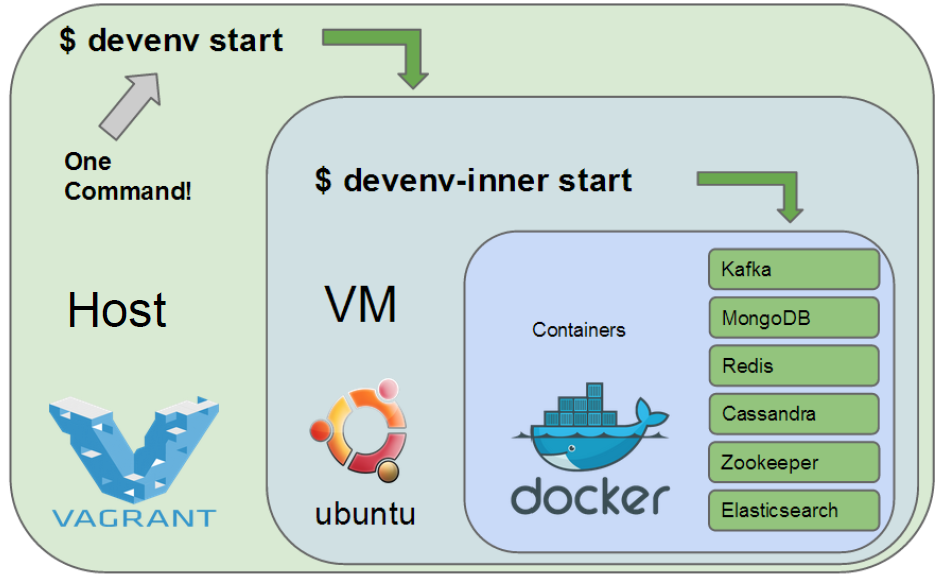
\includegraphics[scale=0.4]{img/integratevagrantdocker.png}
	\caption{Integracja maszyn wirtualnych i kontenerów \cite{ociweb}}
	\label{integrateVagrantDocker}
\end{figure}

\subsection{Struktura obrazów Dockera}

Kontenery są przechowywane w postaci obrazów. Tworzenie nowych obrazów jest możliwe poprzez edycję, czyli dodawanie kolejnych warstw do już istniejących obrazów lub z wykorzystaniem Dockerfile – metoda analogiczna do tworzenia maszyn wirtualnych w oparciu o Vagrantfile, rozszerzona o pobieranie kodu aplikacji bezpośrednio z repozytorium, który jest następnie kompilowany w obrębie kontenera. Każdy krok opisany w Dockerfile, w tym pobranie i kompilacja kodu, tworzy nową warstwę, która rozszerza istniejący obraz. Ponadto istnieje możliwość tworzenia połączeń między kontenerami, co ułatwia korzystanie z poszczególnych modułów aplikacji (np. bazy danych). Docker pozwala na współdzielenie zasobów ze światem zewnętrznym, dzięki czemu aplikacje mogą przetwarzać pliki udostępniane również innym systemom.

\section{CoreOS}

Podstawową różnicą pomiędzy CoreOS \ref{coreOS}, a innymi systemami operacyjnymi z rodziny UNIX jest to, że instalację pakietów oprogramowania zastąpiono włączaniem kolejnych kontenerów Docker do ekosystemu systemu operacyjnego. CoreOS składa się z trzech głównych komponentów:

\begin{itemize}
\item narzędzia odkrywania usług etcd,
\item silnika Docker,
\item manager'a systemu i usług dla środowiska
Linux systemd.
\end{itemize}

\begin{figure}[h] \centering %H if want to get it exaclty here
	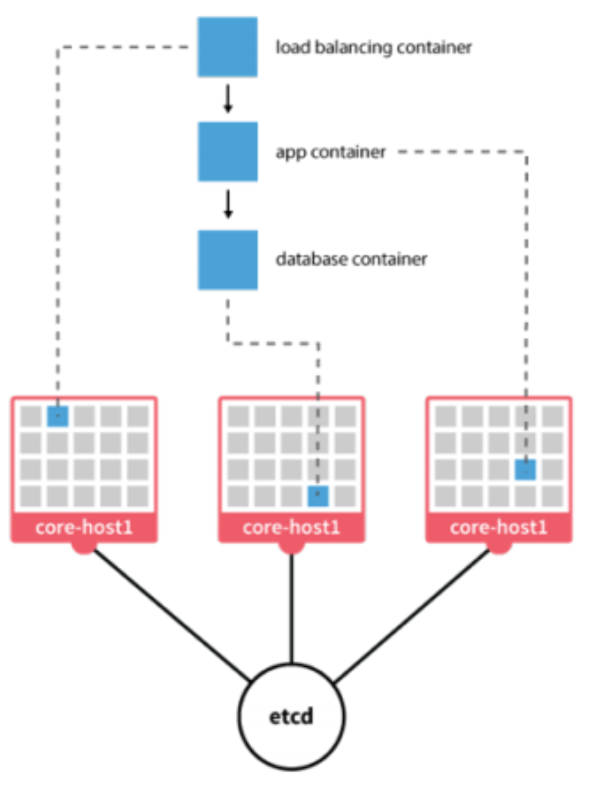
\includegraphics{img/coreOS.png}
	\caption{Struktura CoreOS\cite{coreOS}}
	\label{coreOS}
\end{figure}

Rysunek \ref{coreOS} przedstawia architekturę, w której kontenery z poszczególnymi modułami aplikacji zostają umieszczone na różnych maszynach w oparciu o informacje zawarte w plikach systemd. Nawiązanie komunikacji pomiędzy komponentami następuje z wykorzystaniem narzędzia etcd.

\subsection{Odkrywanie usług z wykorzystaniem etcd}

CoreOS został stworzony i zaprojektowany z myślą o rozproszonych systemach informa- tycznych, co zrodziło zapotrzebowanie dyna- micznego odkrywania usług wystawianych przez aplikacje. Każdy z hostów udostępnia port usłudze etcd, która jest stosowana nie tylko do odkrywania usług, ale również odczytu i zapisu danych konfiguracyjnych. Zamiast umieszczać w kodzie informację o topologii aplikacji (np. bazie danych) wystarczy, że wykorzystamy etcd do ustalenia szczegółów wymaganego połączenia. Moduł aplikacji rejestruje się w usludze etcd podając klucz, który następnie będzie używany przy mapowaniu zapytań typu REST, oraz przypisaną mu wartość (np. klucz „/database” i odpowiadający mu adres bazy danych). Następnie zachodzi replikacja danych konfiguracyjnych w obrębie klastra, dzięki czemu aplikacje uruchomine na różnych maszynach mają lokalny dostęp do aktualnych informacji.

\subsection{Tworzenie klastra kontenerów w oparciu o pliki systemd i narzędzie Fleet}

Pliki systemd opisują poszczególne jednostki wchodzące w skład klastra. W tych opisach można zawrzeć deklracje konfliktów pomiędzy poszczególnymi modułami aplikacji, a także preferencje co do rozmieszczenia tych modułów (np. wymaganie, aby kontener zawierający bazę danych został umieszczony na innej maszynie niż ta, która przechowuje jej backup). Następnie w oparciu o informacje zawarte w plikach systemd następuje przydzielenie kontenerów do konkretnych fizycznych maszyn. Ma to zastosowanie w przypadku usług, które muszą się charakteryzować wysoką dostępnością. W takim wypadku kontenery przechowujące aplikację zostaną umieszczone na niezależnych maszynach, które dodatkowo mogą znajdować się w różnych regionach.

	\bibliographystyle{unsrt}
	\bibliography{sample} 
	\begin{appendices}
		\chapter{Załączniki}
		\begin{description}
			\item \textbf{RxConcurrency} \\
			Aplikacja służąca do obliczenia liczby Pi z dokładnością do podanej liczby miejsc po przecinku. \\
			Pokazująca możliwości paradygmatu reaktywnego w kwestiach współbieżności. \\
			Wykorzystane narzędzia: ReactiveX
			\item \textbf{RxPath} \\
			Aplikacja służąca do rysowania ścieżki na ekranie. \\
			Pokazująca możliwości paradygmatu reaktywnego w obsłudze zdarzeń. \\
			Wykorzystane narzędzia: ReactiveX, SodiumFRP
			\item \textbf{RxProcessing}\\ 
			Aplikacja służąca do zliczania linii z literą 'a' i 'b' w podanym pliku.\\
			Pokazująca możliwości paradygmatu reaktywnego w przetwarzaniu danych. \\
			Wykorzystane narzędzia: ReactiveX, Apache Spark
			\item \textbf{RxSolarsystem} \\
			Aplikacja symulująca Układ Słoneczny. \\
			Pokazująca nowe możliwości w tworzeniu architektury oprogramowania.  \\
			Wykorzystane narzędzia: ReactiveX
		\end{description}
	\end{appendices}
\end{document}

% ex: set tabstop=4 shiftwidth=4 softtabstop=4 noexpandtab fileformat=unix filetype=tex spelllang=pl,en spell:






